
\FloatBarrier
\section{Система Sprott~A}  % {{{1
\label{atu:sect:spr_a}

\LinkRef{
  spr\_a: MKMM-2016
}

\subsection{Визначення системи та аналіз її динаміки} %% {{{2_SPR_task

У своїх роботах J.C.~Sprott розглянув ціле сімейство
динамічних систем, що реалізують хаотичну поведінку,
визначивши їх латинськими буквами від ``A'' до ``S''~\cite{sprott_212,sprott_strange_attr}.
Особливе місце серед них займає система, що позначається як ``Sprott~A''.
Відмінною особливістю цієї системи є відсутність положень рівноваги, що унеможливлює
застосування багатьох відомих методів аналізу, заснованих на будь-якому
розкладі в околі точок рівноваги.
Відповідна їй система рівнянь має вигляд:
%
\begin{equation}
  \begin{cases}
    \dot{x} =  y, \\
    \dot{y} = -x + yz, \\
    \dot{z} =  1 - y^2.
  \end{cases}
  \label{atu:eq:spr_a_orig}
\end{equation}


У початковому вигляді система (\ref{atu:eq:spr_a_orig}) має фіксовані
значення параметрів. Не змінюючи структури системи, можна
ввести 5 параметрів, що впливають на її динамку. Оскільки метою
даної роботи є визначення можливості застосування різних
критеріїв ідентифікації параметрів хаотичних об'єктів, а
також властивостей методів ідентифікації, то для даної системи
розглянемо тільки один параметр ---
$c_{x_y}$. Система приймає наступний вигляд:
%
\begin{equation}
  \begin{cases}
    \dot{x} =  c_{x_y} y, \\
    \dot{y} = -x + yz, \\
    \dot{z} =  1 - y^2.
  \end{cases}
  \label{atu:eq:spr_a}
\end{equation}

У такому вигляді система, при зміні $c_{x_y}$ в досить широкому діапазоні
демонструє як складно-періодичну (рис.~\ref{atu:f:spr_a_p_0372}),
так і переважно хаотичну поведінку (рис.~\ref{atu:f:spr_a_p_0610}).


\begin{figure}[htb!]
\begin{center}
  ~ \hfill
  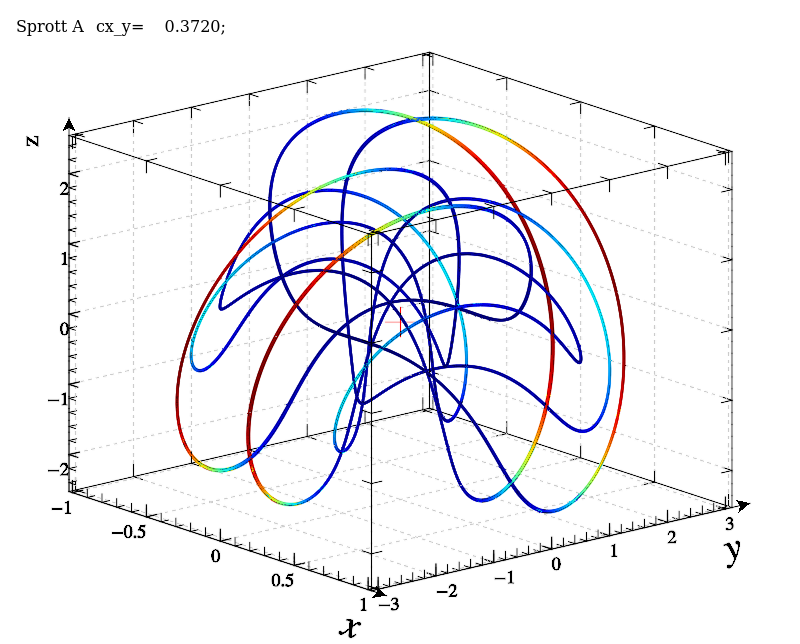
\includegraphics[width=0.49\textwidth]{p/cha/spr_a/sprott_a-p_xyz_cx_y=0x372.png}
  \hfill
  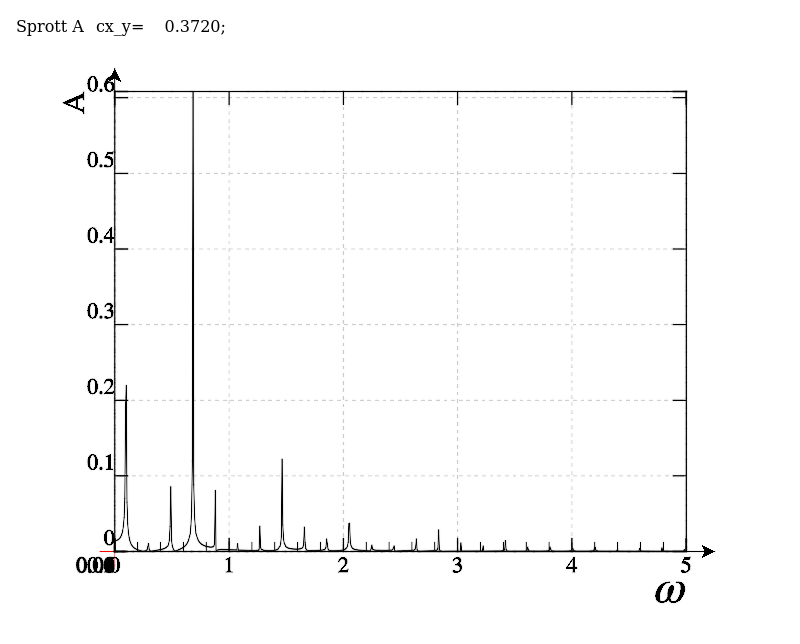
\includegraphics[width=0.49\textwidth]{p/cha/spr_a/sprott_a_f-p_f_cx_y=0x372.png}
  \hfill ~
\end{center}
\vspace{-1.5ex}
\begin{center}
  ~ \hfill a \hfill\hfill b \hfill ~
\end{center}
\vspace{-2.0ex}
\caption{Аттрактор (a) та спектр (b) системи (\ref{atu:eq:spr_a}) при $c_{x_y} =0.372$}
\label{atu:f:spr_a_p_0372}
\end{figure}

При цьому, в діапазоні
$c_{x_y} \in [0.1; 0.7]$ спостерігаються перебудови структури аттрактора,
а при відносно великих значеннях цього параметра аттрактор
являє собою порожнистий тор.

\begin{figure}[htb!]
\begin{center}
  ~ \hfill
  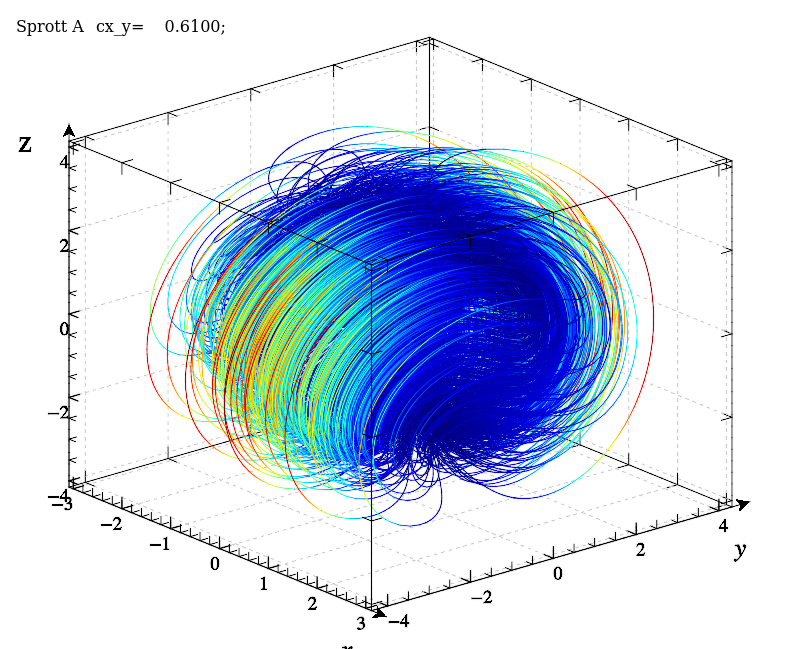
\includegraphics[width=0.49\textwidth]{p/cha/spr_a/sprott_a-p_xyz_cx_y=0x610.png}
  \hfill
  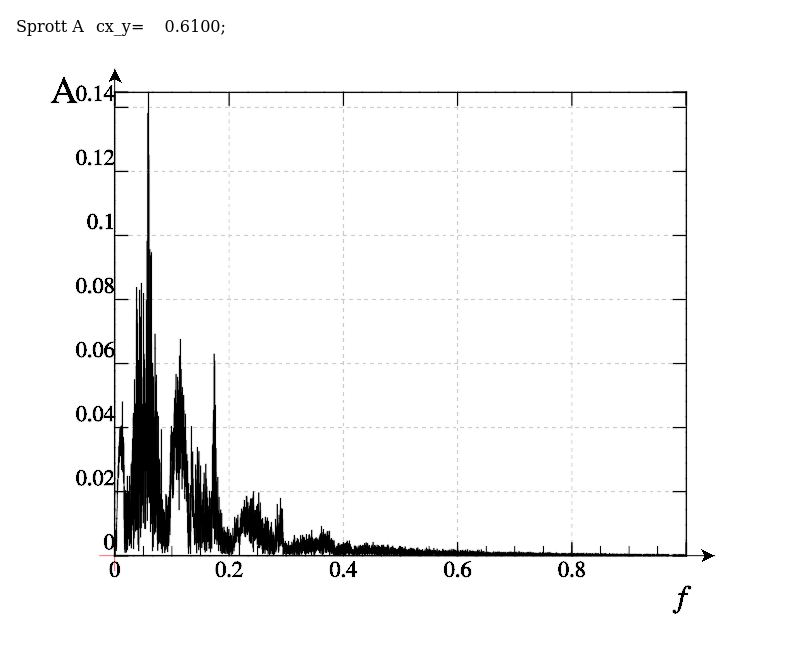
\includegraphics[width=0.49\textwidth]{p/cha/spr_a/sprott_a_f-p_f_cx_y=0x610.png}
  \hfill ~
\end{center}
\vspace{-1.5ex}
\begin{center}
  ~ \hfill a \hfill\hfill b \hfill ~
\end{center}
\vspace{-2.0ex}
\caption{Аттрактор (a) та спектр (b) системи (\ref{atu:eq:spr_a}) при $c_{x_y} =0.610$}
\label{atu:f:spr_a_p_0610}
\end{figure}




Важливою особливістю поведінки цієї системи є те, що при
$c_{x_y} \ge 1$ в спектрі системи є дуже обмежені ділянки суцільного
спектра~(рис.~\ref{atu:f:spr_a_p_1000}). При цьому, як і для отримання
коректного спектра, так і для виявлення ``розбігання'' траєкторій
необхідно моделювання системи протягом досить тривалого (в
порівнянні з багатьма подібними системами) модельного часу.

\begin{figure}[htb!]
\begin{center}
  ~ \hfill
  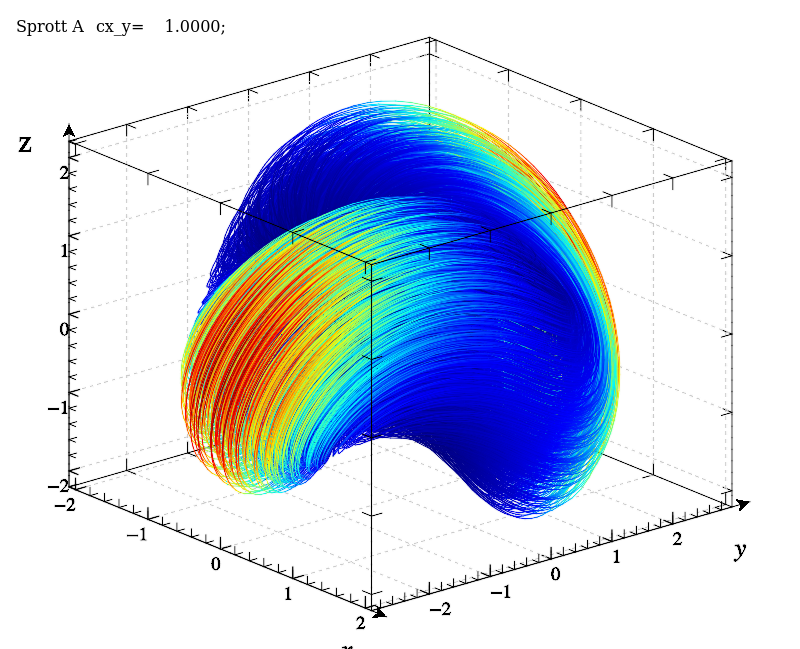
\includegraphics[width=0.49\textwidth]{p/cha/spr_a/sprott_a-p_xyz_cx_y=1x000.png}
  \hfill
  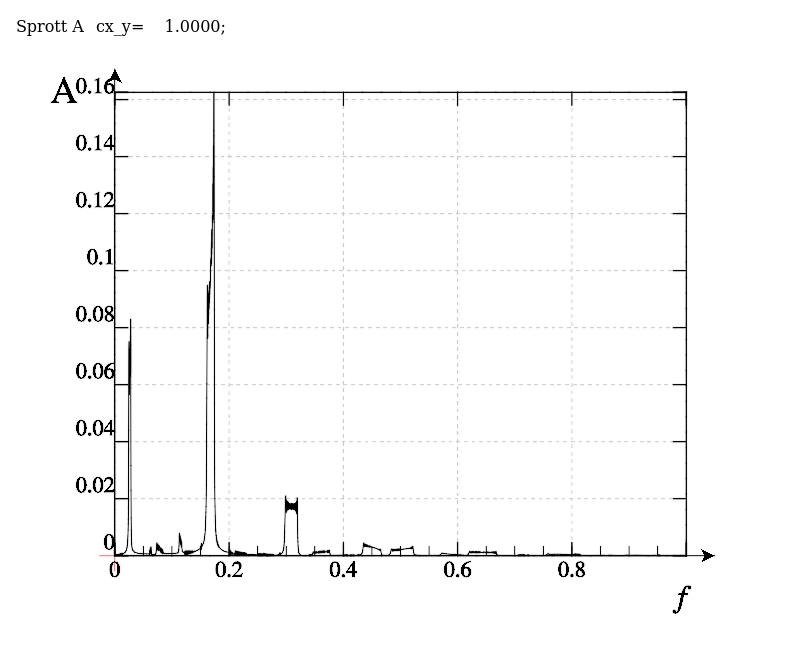
\includegraphics[width=0.49\textwidth]{p/cha/spr_a/sprott_a_f-p_f_cx_y=1x000.png}
  \hfill ~
\end{center}
\vspace{-1.5ex}
\begin{center}
  ~ \hfill a \hfill\hfill b \hfill ~
\end{center}
\vspace{-2.0ex}
\caption{Аттрактор (a) та спектр (b) системи (\ref{atu:eq:spr_a}) при $c_{x_y} =1.0$}
\label{atu:f:spr_a_p_1000}
\end{figure}

% }}}2


\subsection{Аналіз і вибір критеріїв}%{{{2

В першу чергу, на аналогії з системою Лоренца, перевіримо
можливість застосування енергетичних критеріїв, так як існують
реальні фізичні системи, для моделювання яких застосовується
система~(\ref{atu:eq:spr_a_orig}).

Розглянемо залежності
$q_{*} (c_{x_y})$ (рис.~\ref{atu:f:spr_a_q}) для системи (\ref{atu:eq:spr_a}). Аналіз цих
залежностей дає практично однозначну відповідь про можливі
вигляді критерію ---
$q_{x^2}$. Другий кандидат ---
$q_{x}$ --- має меншу лінійність. Також слід зазначити, що значення
критеріїв, в які не входить
$x$, практично не залежать від
$c_{x_y}$, а вид критеріїв
$q_{xy}$ і
$q_{xz}$ нічим не краще, ніж у
$q_{x}$. Таким чином, систему ідентифікації будемо будувати,
використовуючи критерій~$q_{x^2}$~\cite{atu_kher2016}.

\begin{figure}[htb!]
\begin{center}
  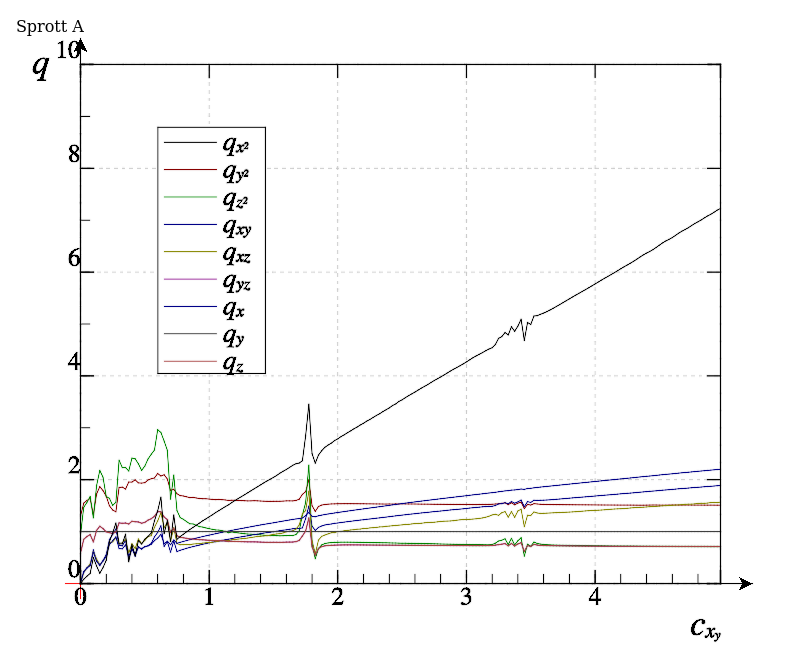
\includegraphics[width=0.60\textwidth]{p/cha/spr_a/sprott_a_q-p_c_x_y.png}
\end{center}
\caption{Залежності $q_{*} (c_{x_y})$ для системи (\ref{atu:eq:spr_a})}
\label{atu:f:spr_a_q}
\end{figure}

Не можна не відзначити, що в початковій області
$q_{x^2} (c_{x_y})$, а саме там, де відбуваються постійні перебудови
структури аттрактора, жоден з розглянутих критеріїв не
має достатньої монотонності, що не дає гарантії побудови
працездатною системи ідентифікації. Для роботи в цій області,
швидше за все, потрібно синтез спеціальних критеріїв.

В околі точки $c_{x_y} = 1.775$ атрактор також різко змінює свою
структуру. Оскільки це досить вузький окіл, то можна припустити, що
мультиагентна система ідентифікації не опиниться непрацездатною в цій області,
лише виросте похибка ідентифікації.

Для проведення ідентифікації було вибрано два сімейства
методів:
ql3rlWvnAAW.$q_{x^2}$ та
Fq3rlFvnAAF.$q_{x^2}$.

Розглянемо залежності, що визначають необхідні інтервали
усереднення критеріїв ідентифікації
--- $\sigma_q(\tau_q)$
або ж
$\sigma_q (a_q)$ --- співвідношення між часом оцінювання
$\tau_q$ і середньоквадратичної похибкою вимірювання критерію.

Для моделювання безпосередніх похибок вимірювання величини
$x (t)$ використовувався шум з нормальним розподілом і
параметрами
$\sigma_w = 0.1$ і
$\tau_w = 0.05$. Для оцінювання необхідної залежності, для кожного
значення
$\tau_q$ з заданого діапазону проводилося
$N = 200$ процесів моделювання динаміки системи, і в випадковий
момент (досить далеко віддалений від точки
$t = 0$ для виключення крайових ефектів) проводилося вимірювання
і запам'ятовування обраного критерію. Так само, як для системи
Лоренца, для усереднення величини
$q$ використовувалося 2 методу: експоненціального згладжування,
виду (\ref{atu:eq:qlin}), і ковзне середнє. Отримані залежності
представлені на рис.~\ref{atu:f:spr_a_qx2_tau}.


\begin{figure}[htb!]
\begin{center}
  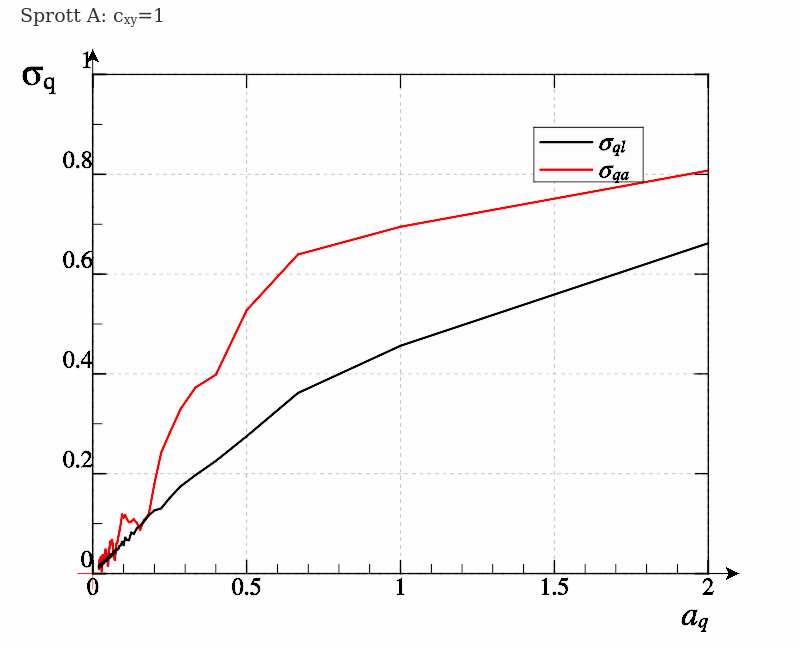
\includegraphics[width=0.49\textwidth]{p/cha/spr_a/sprott_a_qx2_tau-p_aq_sd.png}
  \hfill
  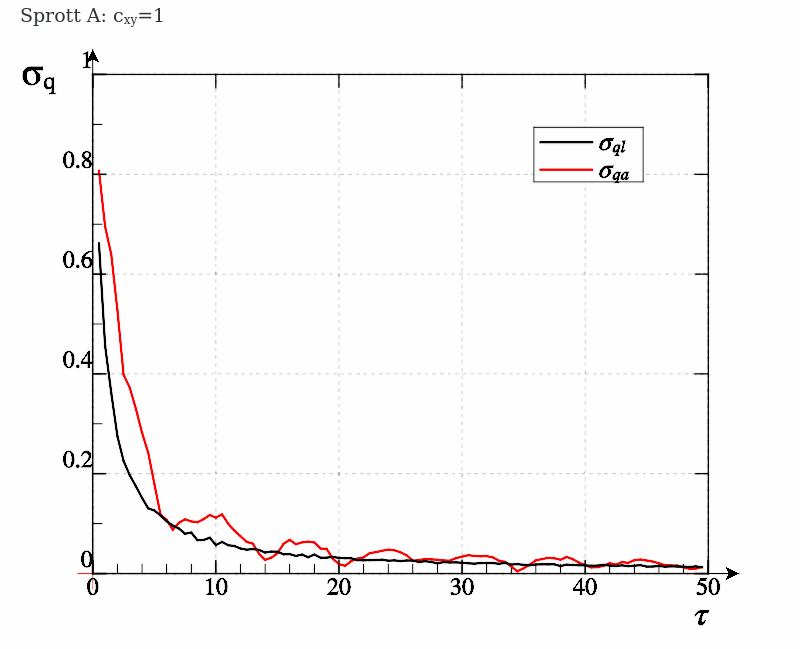
\includegraphics[width=0.49\textwidth]{p/cha/spr_a/sprott_a_qx2_tau-p_tau_sd.png}
\end{center}
\caption{Залежності $\sigma_{q} (a_q)$ і $\sigma_{q} (\tau_q)$ для системи Sprott~A, критерій $q_{x^2}$}
\label{atu:f:spr_a_qx2_tau}
\end{figure}

Вид цих залежностей практично не відрізняється від аналогічних
для системи Лоренца (рис. \ref{atu:f:lor_qx2_tau}). Цілком аналогічно,
ковзне середнє в даних умовах не дає ніяких переваг і не буде
використовуватися далі.

% }}}2


\subsection{Тестова задача ідентифікації для системи Sprott~A} % {{{2

Відповідно до отриманих даних, і використовуючи
пропозиції~(\ref{atu:eq:po_t_sign}) і~(\ref{atu:eq:po_t_sin}),
%
визначимо тестове завдання наступним чином:
\[
  c_{x_y}(t) \equiv p_o(t) \in (0, 5],
\]
%
\begin{equation}
  p_o(t) = p_0 +  U_{p} \sign \sin( \omega_{p} t ),
  \label{atu:eq:spr_a_po_t_sign}
\end{equation}
%
%
\begin{equation}
  p_o(t) = p_0 +  U_{p} \sin( \omega_{p} t ),
  \label{atu:eq:spr_a_po_t_sin}
\end{equation}
%
де:
$p_0 = 2.8$, $U_p=1.9$, $\omega_p=\pi/300$.

На рис.~\ref{atu:f:spr_a_id_ql3rlWvnAAW_q_x2_sign}
представлені результати моделювання процесу ідентифікації групою методів ql3rlWvnAAW.$q_{x^2}$.
Аналогічно системі Лоренца, на лівому графіку зображено
динаміку переміщення кожної з рухливих моделей, а на правому ---
8 способів визначення
$p_\mathrm{id} (t)$.

\begin{figure}[htb!]
 \begin{center}
    ~ \hfill
    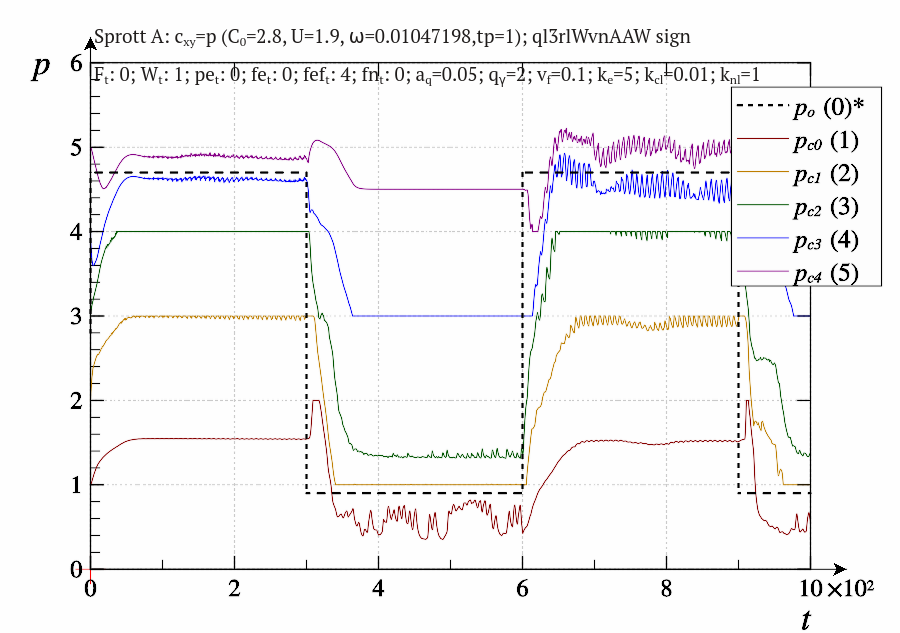
\includegraphics[width=0.49\textwidth]{p/cha/spr_a/ql3rlWvnAAW_x2/sprott_a_id-p_t_pi_ql3rlWvnAAW_sign.png}
    \hfill
    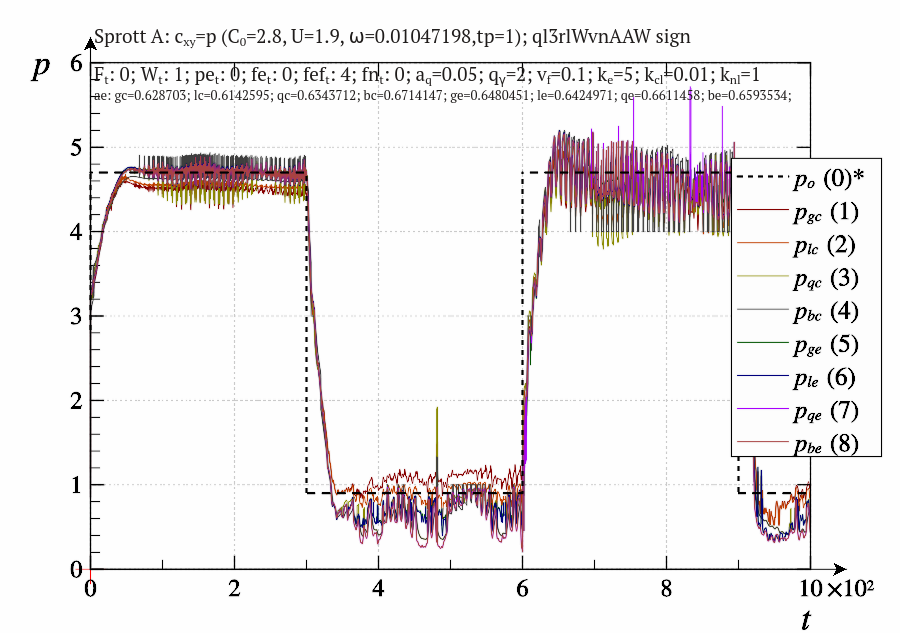
\includegraphics[width=0.49\textwidth]{p/cha/spr_a/ql3rlWvnAAW_x2/sprott_a_id-p_t_p_ql3rlWvnAAW_sign.png}
    \hfill ~
  \end{center}
  \vspace{-2.2ex}
  \begin{center}
    ~ \hfill a \hfill\hfill b \hfill ~
  \end{center}
  \vspace{-1.0ex}
\caption{Процес ідентифікації параметра ``$c_{x_y}$'' системи Sprott~A групою методів ql3rlWvnAAW.$q_{x^2}$ за умови~(\ref{atu:eq:spr_a_po_t_sign}): динаміка агентів~(a) та $p_\mathrm{id}$~(b)}
  \label{atu:f:spr_a_id_ql3rlWvnAAW_q_x2_sign}
\end{figure}

В першу чергу, слід зазначити відмінність між процесами
ідентифікації цим методом даної системи і система Лоренца.
Залежність $p_{gc}(t)$, в даному випадку демонструє високий
рівень коливань, і, отже, гірші результати пошуку. При цьому, інші підходи до
визначення $p_\mathrm{id}$ демонструють схожі між собою результати.
Також слід зазначити, що на третьому напівперіоді рівень
коливань помітно вище, ніж на першому. Аналіз значень критерію
показує, що це обумовлено реакцією об'єкта на стрибкоподібне
зміна параметра.
%$\overline{e}_{bm}=1.41$
%$\overline{e}_{ba}=1.49$.



На рис.~\ref{atu:f:spr_a_id_ql3rlWvnAAW_q_x2_sin} представлені аналогічні
результати, але за умови плавної зміни значення
$p_o(t)$. Також очевидно, що як абсолютні, так і відносні значення
помилок ідентифікації в даному випадку трохи менше, при
збереженні загальної картини.
%$\overline{e}_{bm}=0.91$
%и
%$\overline{e}_{ba}=0.84$.

\begin{figure}[htb!]
\begin{center}
  ~ \hfill
    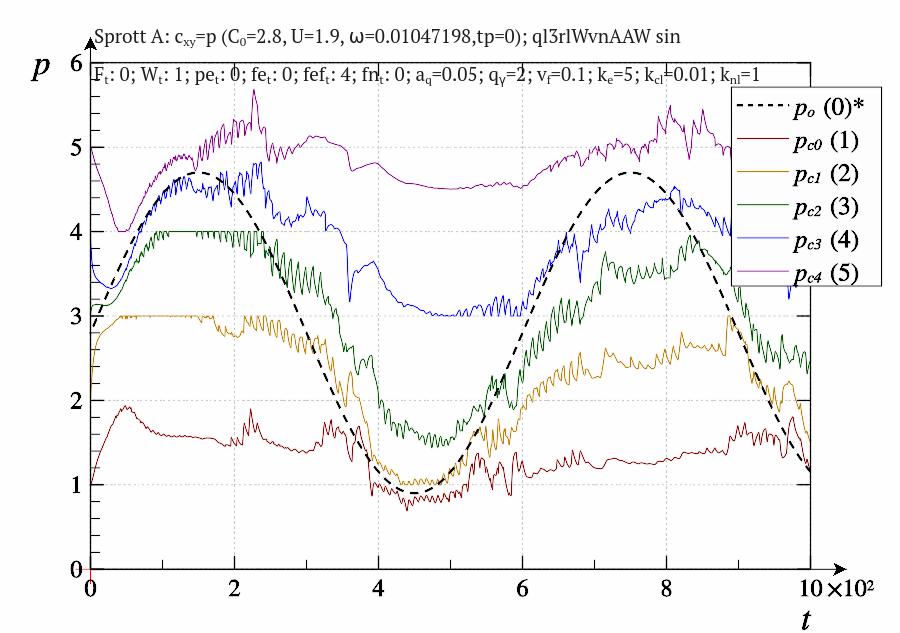
\includegraphics[width=0.49\textwidth]{p/cha/spr_a/ql3rlWvnAAW_x2/sprott_a_id-p_t_pi_ql3rlWvnAAW_sin.png}
    \hfill
    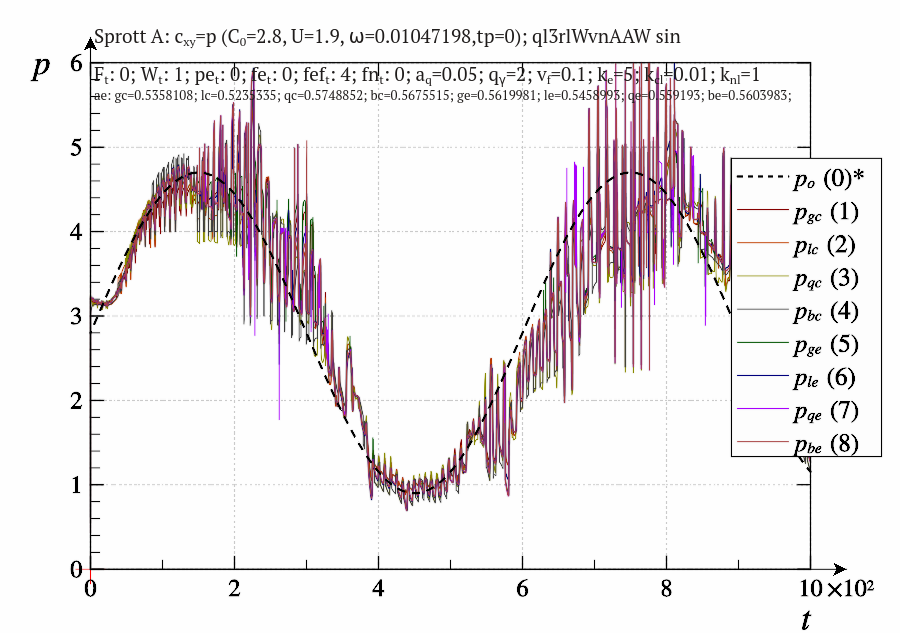
\includegraphics[width=0.49\textwidth]{p/cha/spr_a/ql3rlWvnAAW_x2/sprott_a_id-p_t_p_ql3rlWvnAAW_sin.png}
  \hfill ~
\end{center}
  \vspace{-1.0ex}
  \begin{center}
    ~ \hfill a \hfill\hfill b \hfill ~
  \end{center}
\caption{Процес ідентифікації параметра ``$c_{x_y}$'' системи Sprott~A групою методів ql3rlWvnAAW.$q_{x^2}$ за умови~(\ref{atu:eq:spr_a_po_t_sin}): динаміка агентів~(a) та $p_\mathrm{id}$~(b)}
  \label{atu:f:spr_a_id_ql3rlWvnAAW_q_x2_sin}
\end{figure}

Для перевірки рівномірності похибки ідентифікації на всьому
робочому діапазоні параметра була проведена ідентифікація,
при якій значення параметра плавно пробігало весь діапазон,
тобто використовувалася умова (\ref{atu:eq:po_t_ramp}). Результати
моделювання наведені на рис.~\ref{atu:f:spr_a_id_ql3rlWvnAAW_q_x2_ramp}. Ці
результати дозволяють зробити висновок про те, що у верхній
частині діапазону спостерігається плавне зростання похибки
ідентифікації, що можно було предбачити з виду критерію. Однак, відмічені
локальні обурення критерію не привели до помітних відхилень.


\begin{figure}[htb!]
\begin{center}
  ~ \hfill
    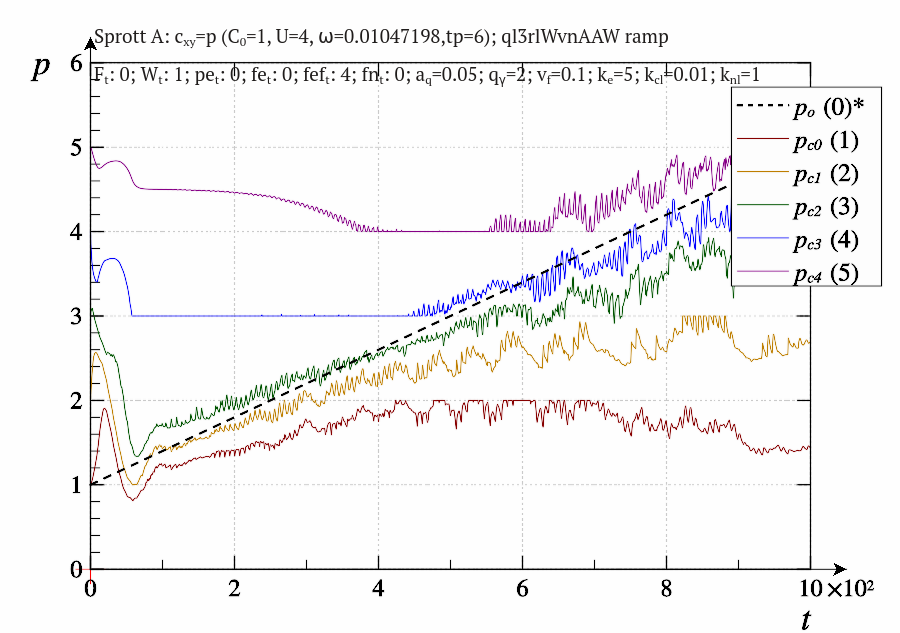
\includegraphics[width=0.49\textwidth]{p/cha/spr_a/ql3rlWvnAAW_x2/sprott_a_id-p_t_pi_ql3rlWvnAAW_ramp.png}
    \hfill
    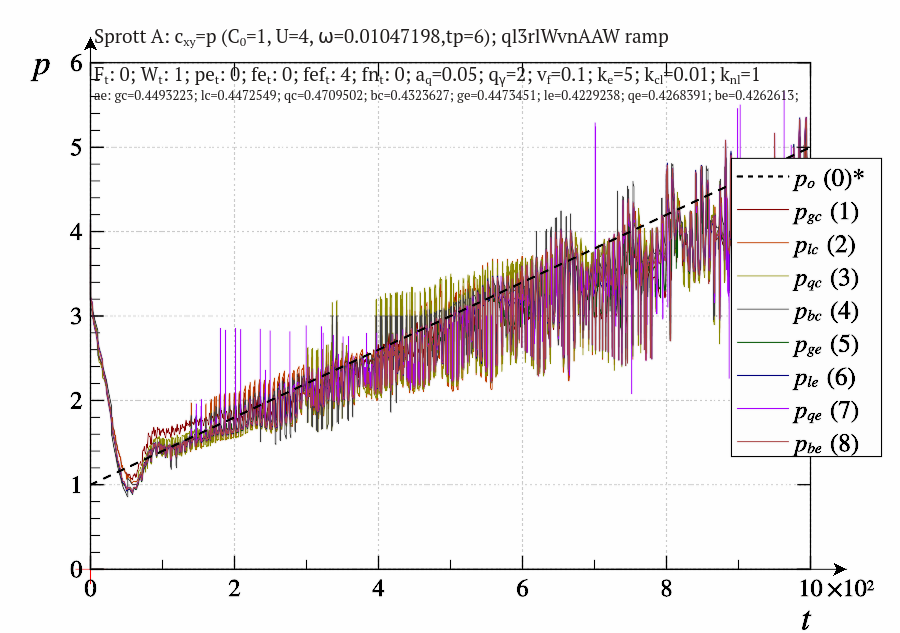
\includegraphics[width=0.49\textwidth]{p/cha/spr_a/ql3rlWvnAAW_x2/sprott_a_id-p_t_p_ql3rlWvnAAW_ramp.png}
  \hfill ~
\end{center}
  \vspace{-1.0ex}
  \begin{center}
    ~ \hfill a \hfill\hfill b \hfill ~
  \end{center}
\caption{Процес ідентифікації параметра ``$c_{x_y}$'' системи Sprott~A групою методів ql3rlWvnAAW.$q_{x^2}$ за умови~(\ref{atu:eq:po_t_ramp}): динаміка агентів~(a) та $p_\mathrm{id}$~(b)}
\label{atu:f:spr_a_id_ql3rlWvnAAW_q_x2_ramp}
\end{figure}

На рис.~\ref{atu:f:spr_a_id_Fq3rlFvnAAF_q_x2_sign} представлені результати
ідентифікації групою методів Fq3rlFvnAAF.$q_{x^2}$. Рівень помилок ідентифікації має практично однакові
значення в порівнянні з групою методів ql3rlWvnAAW. При цьому помітно
більший рівень похибки спостерігається при використанні методу
$p_{gc}$ в процесі роботи координатора пошуку.
% $\overline{e}_{bm}=1.71$


\begin{figure}[htb!]
\begin{center}
  ~ \hfill
    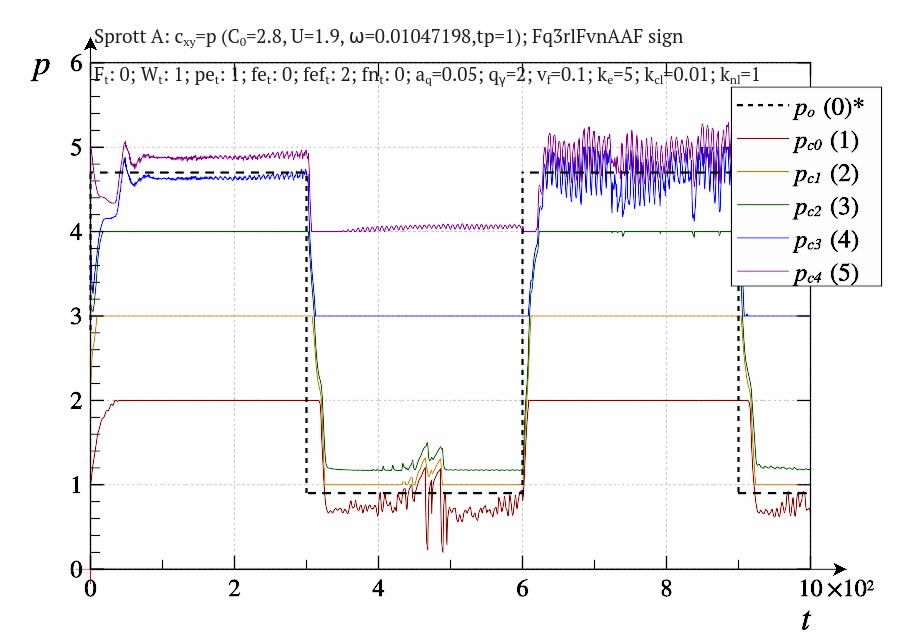
\includegraphics[width=0.49\textwidth]{p/cha/spr_a/Fq3rlFvnAAF_x2/sprott_a_id-p_t_pi_Fq3rlFvnAAF_sign.png}
    \hfill
    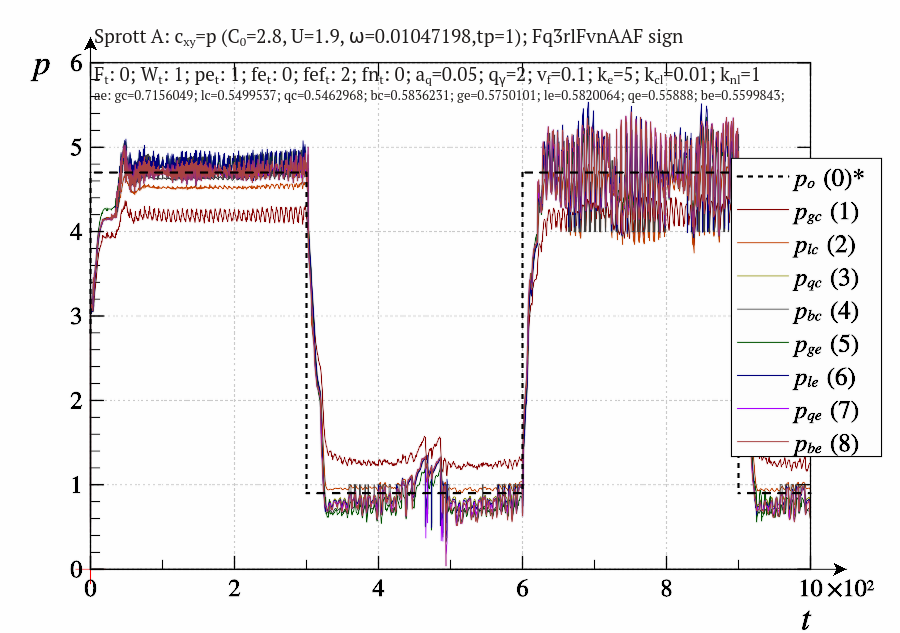
\includegraphics[width=0.49\textwidth]{p/cha/spr_a/Fq3rlFvnAAF_x2/sprott_a_id-p_t_p_Fq3rlFvnAAF_sign.png}
  \hfill ~
\end{center}
  \vspace{-1.0ex}
  \begin{center}
    ~ \hfill a \hfill\hfill b \hfill ~
  \end{center}
\caption{Процес ідентифікації параметра ``$c_{x_y}$'' системи Sprott~A групою методів Fq3rlFvnAAF.$q_{x^2}$ за умови~(\ref{atu:eq:spr_a_po_t_sign})}
  \label{atu:f:spr_a_id_Fq3rlFvnAAF_q_x2_sign}
\end{figure}

На рис.~\ref{atu:f:spr_a_id_Fq3rlFvnAAF_q_x2_sin} представлені аналогічні
результати, але за умови плавної зміни значення параметра
об'єкта. Очевидно, що як абсолютні, так і відносні значення
помилок ідентифікації в даному випадку помітно менше, при
збереженні загальної картини. %
%$\overline{e}_{bm} = 0.87$

\begin{figure}[htb!]
\begin{center}
  ~ \hfill
    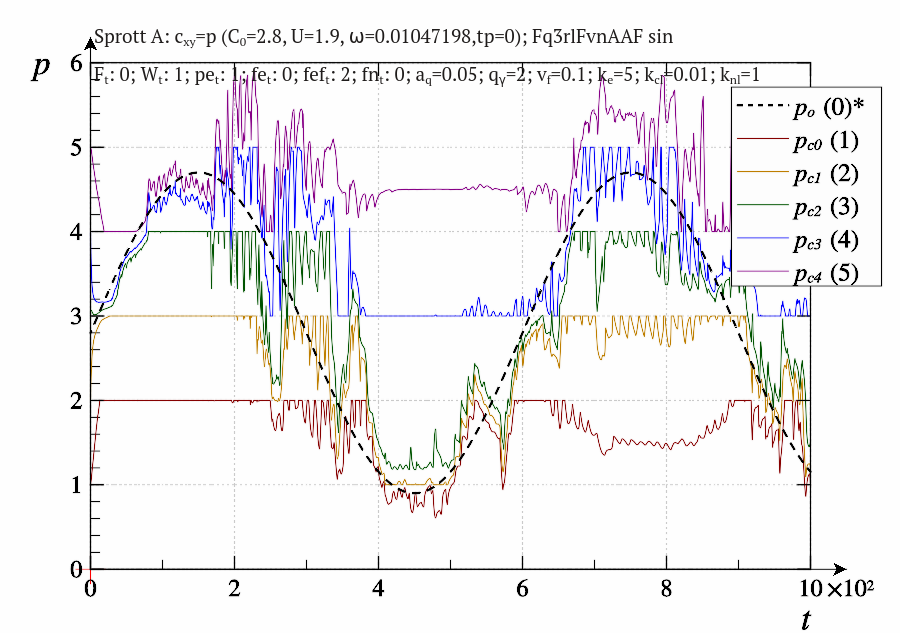
\includegraphics[width=0.49\textwidth]{p/cha/spr_a/Fq3rlFvnAAF_x2/sprott_a_id-p_t_pi_Fq3rlFvnAAF_sin.png}
    \hfill
    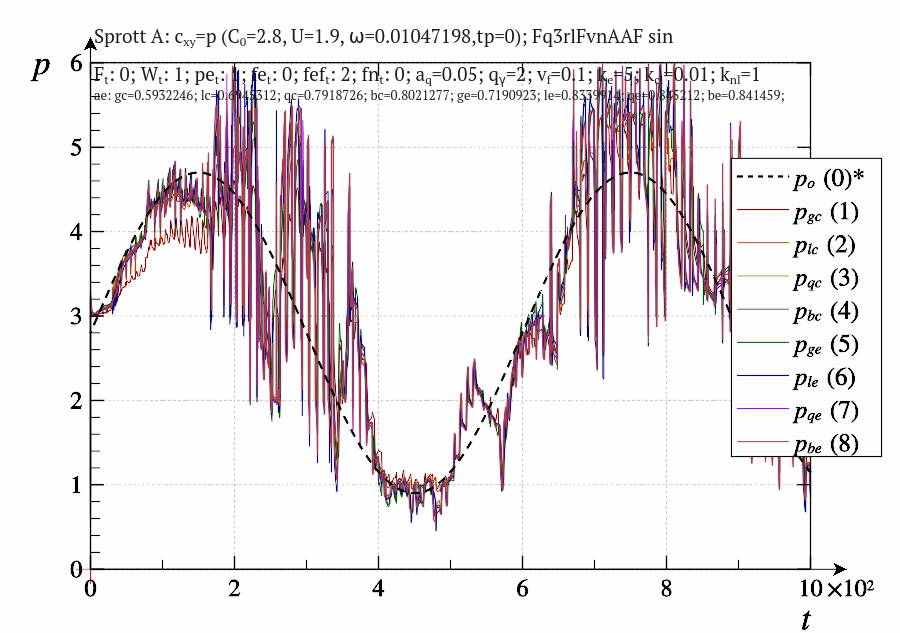
\includegraphics[width=0.49\textwidth]{p/cha/spr_a/Fq3rlFvnAAF_x2/sprott_a_id-p_t_p_Fq3rlFvnAAF_sin.png}
  \hfill ~
\end{center}
  \vspace{-1.0ex}
  \begin{center}
    ~ \hfill a \hfill\hfill b \hfill ~
  \end{center}
\caption{Процес ідентифікації параметра ``$c_{x_y}$'' системи Sprott~A групою методів Fq3rlFvnAAF.$q_{x^2}$ за умови~(\ref{atu:eq:spr_a_po_t_sin}): динаміка агентів~(a) та $p_\mathrm{id}$~(b)}
\label{atu:f:spr_a_id_Fq3rlFvnAAF_q_x2_sin}
\end{figure}

Результати перевірки рівномірності похибки ідентифікації
на всьому робочому діапазоні параметра наведені на
рис.~\ref{atu:f:spr_a_id_Fq3rlFvnAAF_q_x2_ramp}.


\begin{figure}[htb!]
\begin{center}
  ~ \hfill
    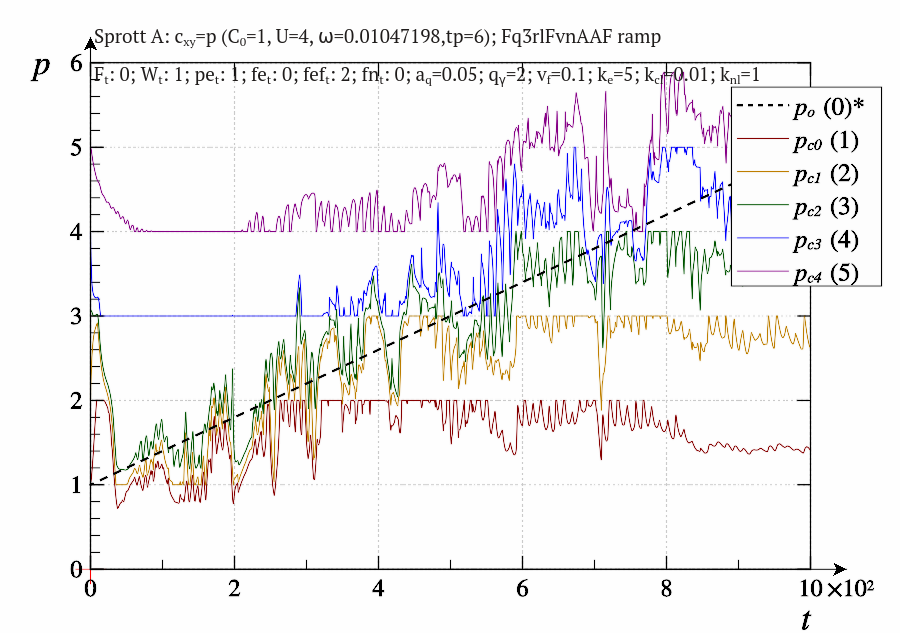
\includegraphics[width=0.49\textwidth]{p/cha/spr_a/Fq3rlFvnAAF_x2/sprott_a_id-p_t_pi_Fq3rlFvnAAF_ramp.png}
    \hfill
    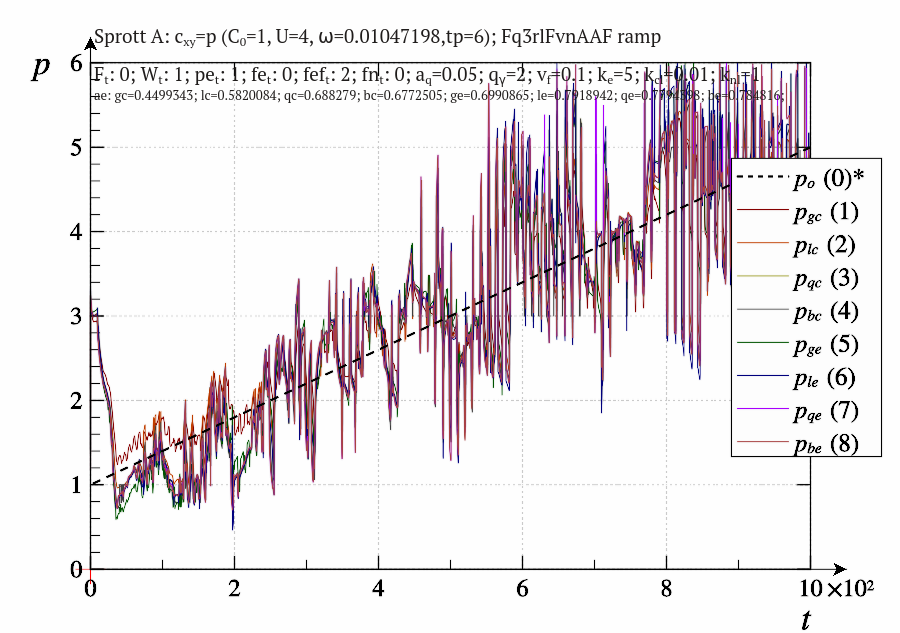
\includegraphics[width=0.49\textwidth]{p/cha/spr_a/Fq3rlFvnAAF_x2/sprott_a_id-p_t_p_Fq3rlFvnAAF_ramp.png}
  \hfill ~
\end{center}
\vspace{-1.5ex}
\begin{center}
  ~ \hfill a \hfill\hfill b \hfill ~
\end{center}
\vspace{-2.5ex}
\caption{Процес ідентифікації параметра ``$c_{x_y}$'' системи Sprott~A групою методів Fq3rlFvnAAF.$q_{x^2}$ за умови~(\ref{atu:eq:po_t_ramp}): динаміка агентів~(a) та $p_\mathrm{id}$~(b)}
  \label{atu:f:spr_a_id_Fq3rlFvnAAF_q_x2_ramp}
\end{figure}

Загальний рівень коливань на цьому графіку не дає можливості
досить коректно оцінити рівномірність рівня похибки при
зміні значення параметра. Однак, в даному обчислювальному
експерименті зберігається працездатність системи
ідентифікації, а група методів Fq3rlFvnAAF в цілому трохи
поступається групі ql3rlWvnAAW.


% }}}2


\subsection{Вплив параметрів системи ідентифікації на похибку ідентифікації для системи Sprott~A} % {{{2


Розглянемо вплив параметрів системи ідентифікації на похибки
ідентифікації.

Перший параметр ---
$a_q$, який визначає характерний час усереднення критерію.

На рис.~\ref{atu:f:spr_a_a_q_ql3rlWvnAAW_q_x2} представлені залежності
$\overline{e} (a_q)$ при застосуванні методу ql3rlWvnAAW.$q_{x^2}$. Вид залежностей аналогічний таким, отриманим для
ідентифікації системи Лоренца~\cite{atu_kher2015}, і визначається він
тими ж факторами, тобто положення екстремуму визначається
балансом між динамічними властивостями самої системи і
динамікою зміни параметра.


\begin{figure}[htb!]
\begin{center}
  ~ \hfill
    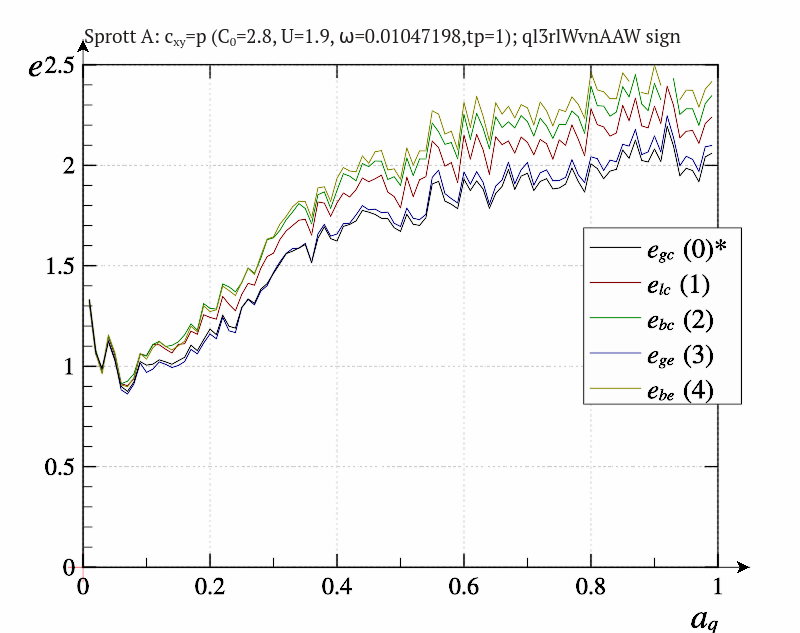
\includegraphics[width=0.49\textwidth]{p/cha/spr_a/ql3rlWvnAAW_x2/sprott_a_id-p_a_q_sign.png}
    \hfill
    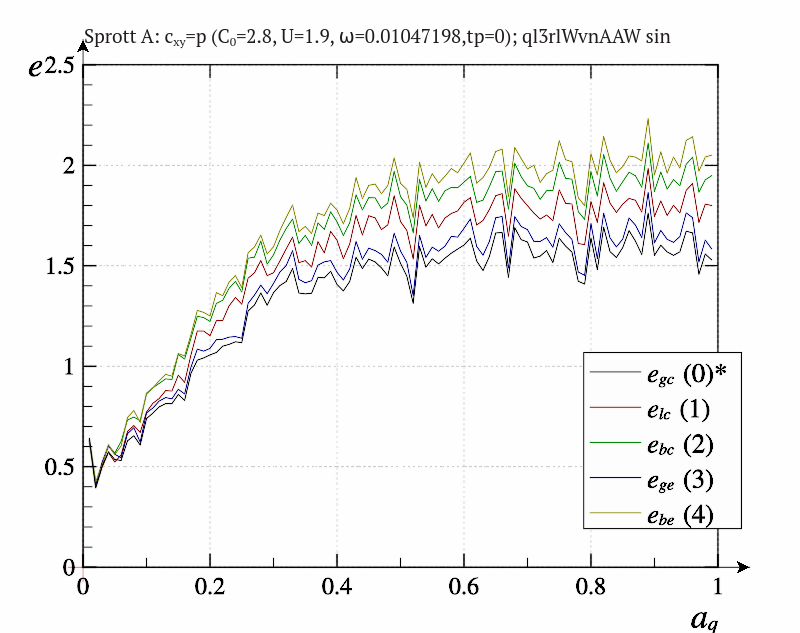
\includegraphics[width=0.49\textwidth]{p/cha/spr_a/ql3rlWvnAAW_x2/sprott_a_id-p_a_q_sin.png}
  \hfill ~
\end{center}
  \vspace{-1.0ex}
  \begin{center}
    ~ \hfill a \hfill\hfill b \hfill ~
  \end{center}
  \caption{Залежності $\overline{e}(a_q)$ при ідентифікації системи Sprott~A групою методів ql3rlWvnAAW.$q_{x^2}$ при~(\ref{atu:eq:spr_a_po_t_sign})~(a) і (\ref{atu:eq:spr_a_po_t_sin})~(b)}
  \label{atu:f:spr_a_a_q_ql3rlWvnAAW_q_x2}
\end{figure}


На рис.~\ref{atu:f:spr_a_a_q_Fq3rlFvnAAF_q_x2} представлені залежності
$\overline{e} (a_q)$ при застосуванні групи методів Fq3rlFvnAAF.$q_{x^2}$.
І в цьому випадку отримані результати, які не
вибиваються із загального ряду. Мінімальні значення помилок
ідентифікації практично збігаються з такими при застосуванні
попереднього методу, а необхідний час усереднення критерію
дещо більше. Незважаючи на це, за інших рівних даний метод
забезпечує дещо більший рівень коливання
$p_\mathrm{id}$ в процесі пошуку.


\begin{figure}[htb!]
\begin{center}
  ~ \hfill
    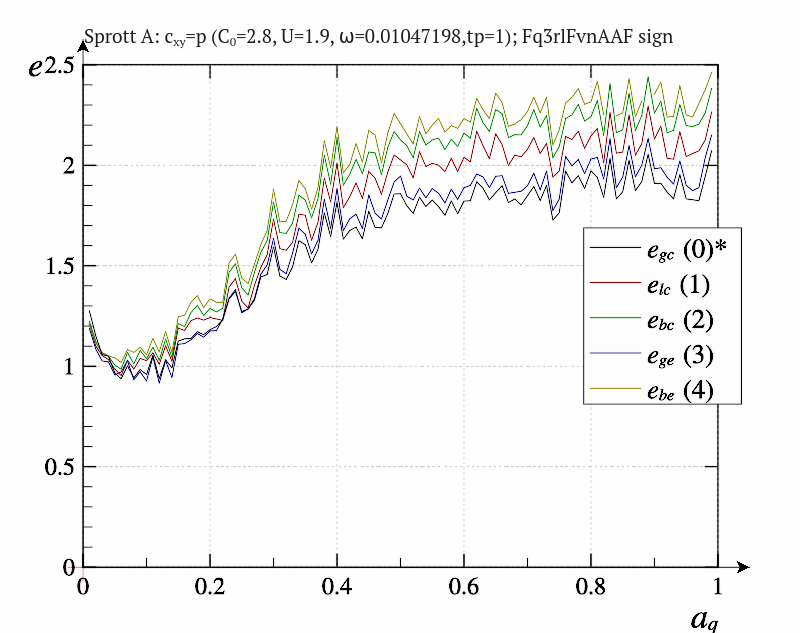
\includegraphics[width=0.49\textwidth]{p/cha/spr_a/Fq3rlFvnAAF_x2/sprott_a_id-p_a_q_sign.png}
    \hfill
    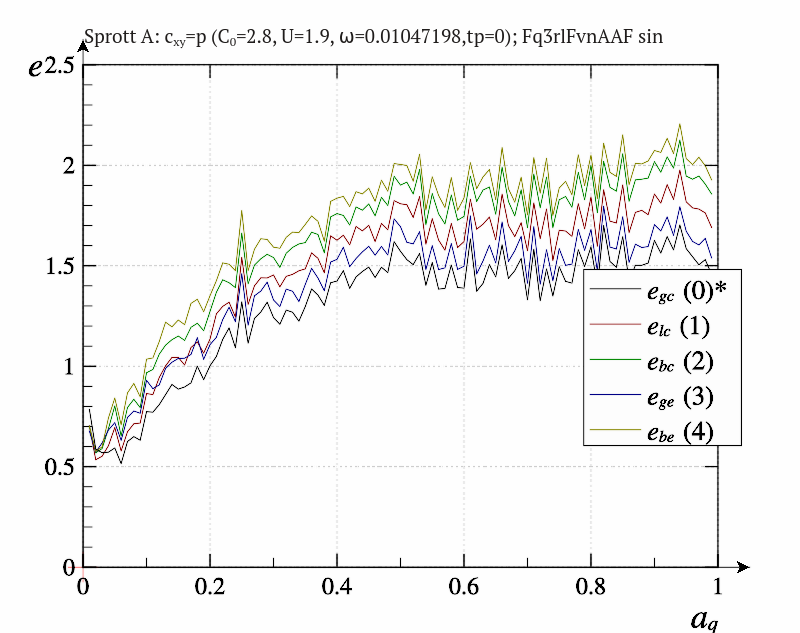
\includegraphics[width=0.49\textwidth]{p/cha/spr_a/Fq3rlFvnAAF_x2/sprott_a_id-p_a_q_sin.png}
  \hfill ~
\end{center}
  \vspace{-1.0ex}
  \begin{center}
    ~ \hfill a \hfill\hfill b \hfill ~
  \end{center}
  \caption{Залежності $\overline{e}(a_q)$ при ідентифікації системи Sprott~A групою методів Fq3rlFvnAAF.$q_{x^2}$ при~(\ref{atu:eq:spr_a_po_t_sign})~(a) і (\ref{atu:eq:spr_a_po_t_sin})~(b)}
  \label{atu:f:spr_a_a_q_Fq3rlFvnAAF_q_x2}
\end{figure}

Наступний параметр ---
$q_\gamma$ повинен чинити більший вплив на процеси ідентифікації,
що використовують для оцінки
$p_e$ функцію якості.

На рис.~\ref{atu:f:spr_a_ql3rlWvnAAW_q_x2} представлені залежності
$\overline{e} (q_\gamma)$ при застосуванні групи методів ql3rlWvnAAW.$q_{x^2}$.
Зростання помилок ідентифікації при зростанні
$q_\gamma <2$ прогнозуємо, при цьому різні способи оцінювання
$p_\mathrm{id}$ дають практично неможливо розрізнити результати.

\begin{figure}[htb!]
\begin{center}
  ~ \hfill
    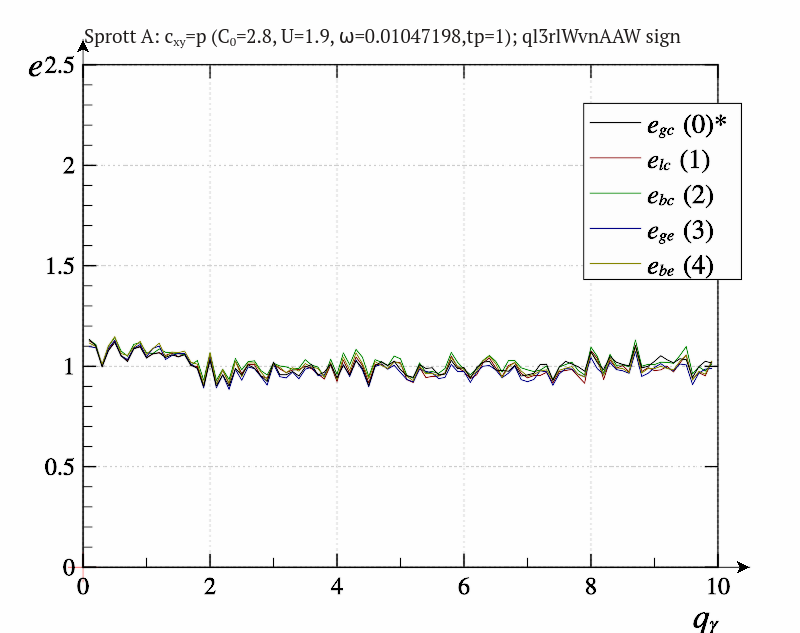
\includegraphics[width=0.49\textwidth]{p/cha/spr_a/ql3rlWvnAAW_x2/sprott_a_id-p_q_gamma_sign.png}
    \hfill
    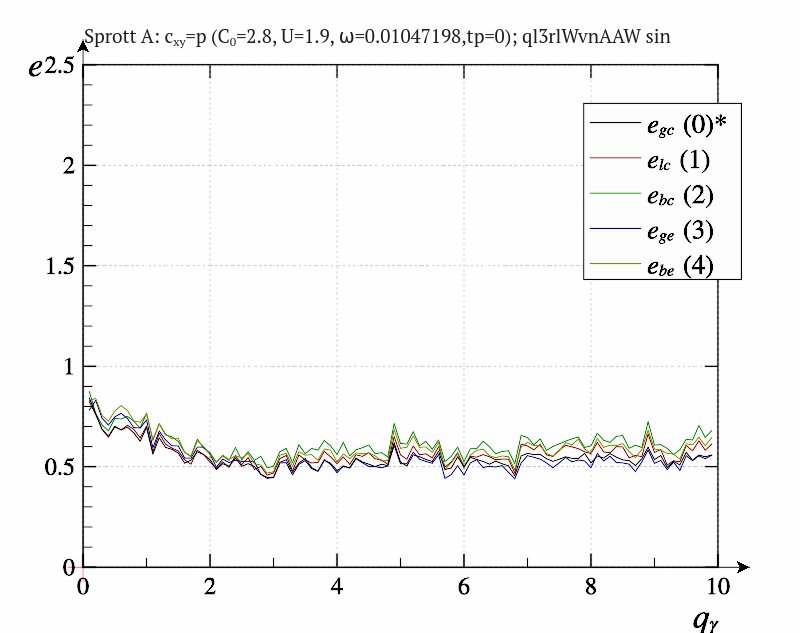
\includegraphics[width=0.49\textwidth]{p/cha/spr_a/ql3rlWvnAAW_x2/sprott_a_id-p_q_gamma_sin.png}
  \hfill ~
\end{center}
  \vspace{-1.0ex}
  \begin{center}
    ~ \hfill a \hfill\hfill b \hfill ~
  \end{center}
  \caption{Залежності $\overline{e} (q_\gamma)$ при ідентифікації системи Sprott~A групою методів ql3rlWvnAAW.$q_{x^2}$ при~(\ref{atu:eq:spr_a_po_t_sign})~(a) і (\ref{atu:eq:spr_a_po_t_sin})~(b)}
  \label{atu:f:spr_a_ql3rlWvnAAW_q_x2}
\end{figure}

На рис.~\ref{atu:f:spr_a_qg_Fq3rlFvnAAF_q_x2} представлені залежності
$\overline{e} (q_\gamma)$ при застосуванні методів Fq3rlFvnAAF.$q_{x^2}$.
Знову ж таки, спостерігається повна
аналогія. Відмінність від системи Лоренца спостерігається
тільки в лівій частині графіка, де зростання помилок при малих
значеннях
$q_\gamma$ замаскований великим загальним рівнем похибки
ідентифікації. Для даної системи розглянутий діапазон
недостатній для спостереження цього ефекту, і зростання похибки
ідентифікації спостерігається тільки при досить малих його
значеннях.

\begin{figure}[htb!]
\begin{center}
  ~ \hfill
    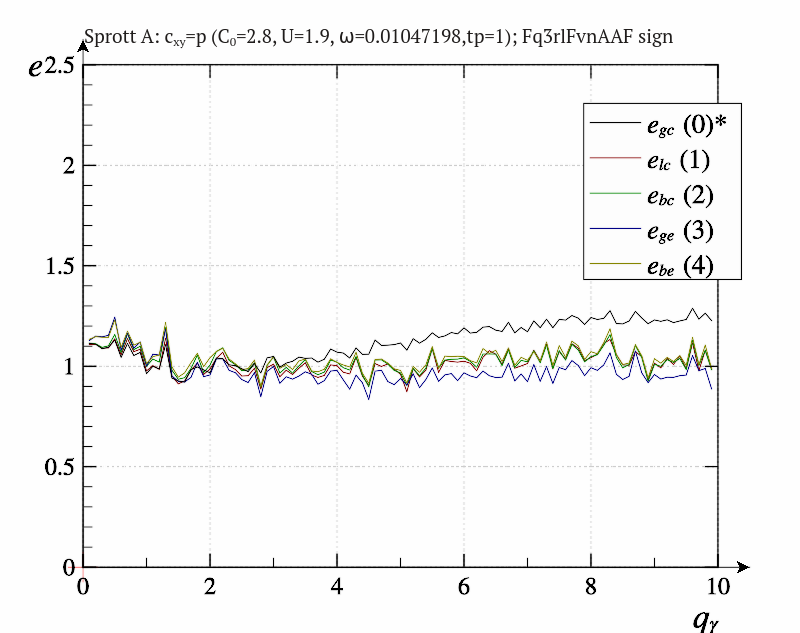
\includegraphics[width=0.49\textwidth]{p/cha/spr_a/Fq3rlFvnAAF_x2/sprott_a_id-p_q_gamma_sign.png}
    \hfill
    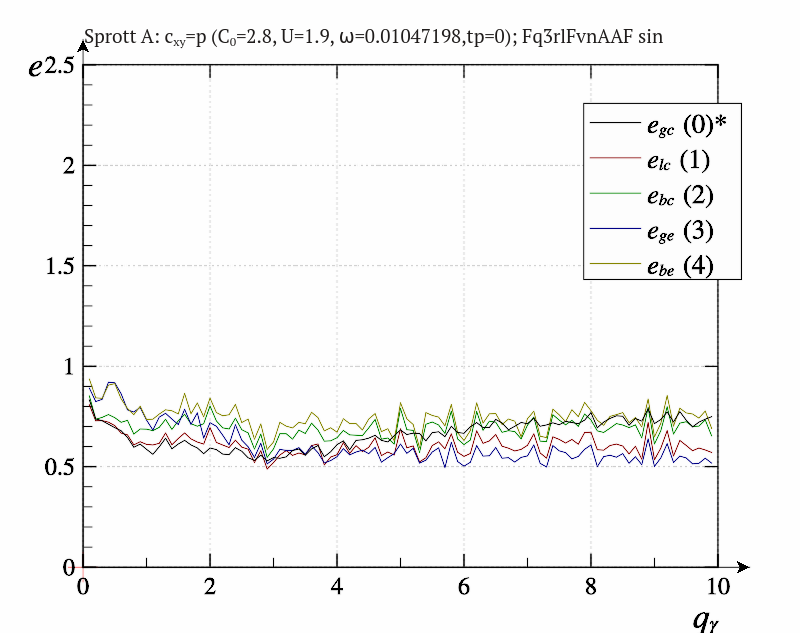
\includegraphics[width=0.49\textwidth]{p/cha/spr_a/Fq3rlFvnAAF_x2/sprott_a_id-p_q_gamma_sin.png}
  \hfill ~
\end{center}
  \vspace{-1.0ex}
  \begin{center}
    ~ \hfill a \hfill\hfill b \hfill ~
  \end{center}
  \caption{Залежності $\overline{e} (q_\gamma)$ при ідентифікації системи Sprott~A групою методів Fq3rlFvnAAF.$_{x^2}$ при~(\ref{atu:eq:spr_a_po_t_sign})~(a) і (\ref{atu:eq:spr_a_po_t_sin})~(b)}
  \label{atu:f:spr_a_qg_Fq3rlFvnAAF_q_x2}
\end{figure}

В цілому, для даної системи залежності
$\overline{e}(q_\gamma)$ свідчать про досить слабкий вплив цього
параметра на динаміку системи ідентифікації. Виявляються
робастні властивості пошукових агентів, і для групи методів
ql3rlWvnAAW ці властивості проявляються сильніше.


Розглянемо вплив параметра
$v_f$, що визначає динаміку пошукових агентів.

На рис.~\ref{atu:f:spr_a_v_f_ql3rlWvnAAW_q_x2} представлені залежності
$\overline{e} (v_f)$ при застосуванні групи методів ql3rlWvnAAW.$q_{x^2}$.
Залежності практично відсутні. Це свідчить про те, що зміщення
пошукових агентів в процесі пошуку для даної системи не має
практично ніякого сенсу. Швидше за все, це пов'язано з тим, що в
даній постановці час реакції системи на стрибкоподібні зміни
параметра має той же порядок, що і необхідний час оцінювання
параметра, що робить пошук практично марним. Зростання помилок
ідентифікації на правому графіку обумовлений надлишковою
динамікою пошукових агентів.



\begin{figure}[htb!]
\begin{center}
  ~ \hfill
    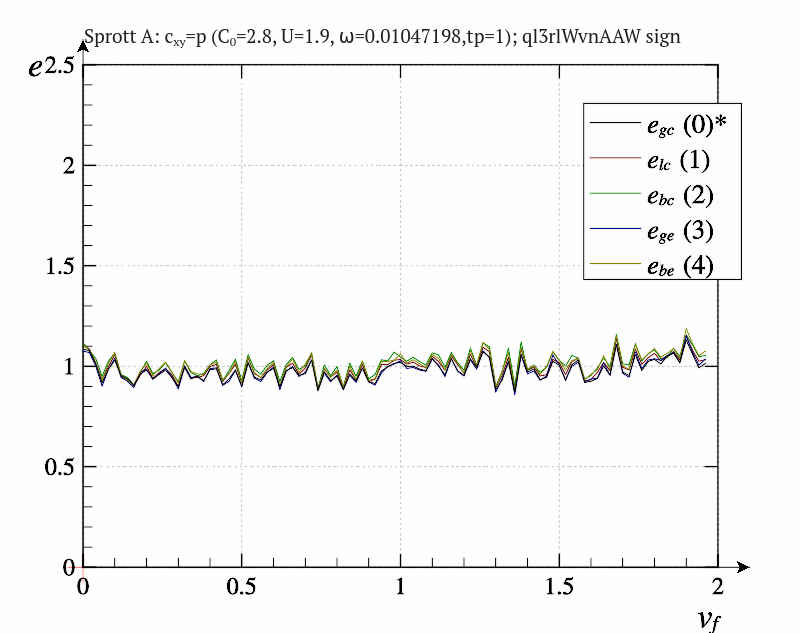
\includegraphics[width=0.49\textwidth]{p/cha/spr_a/ql3rlWvnAAW_x2/sprott_a_id-p_v_f_sign.png}
    \hfill
    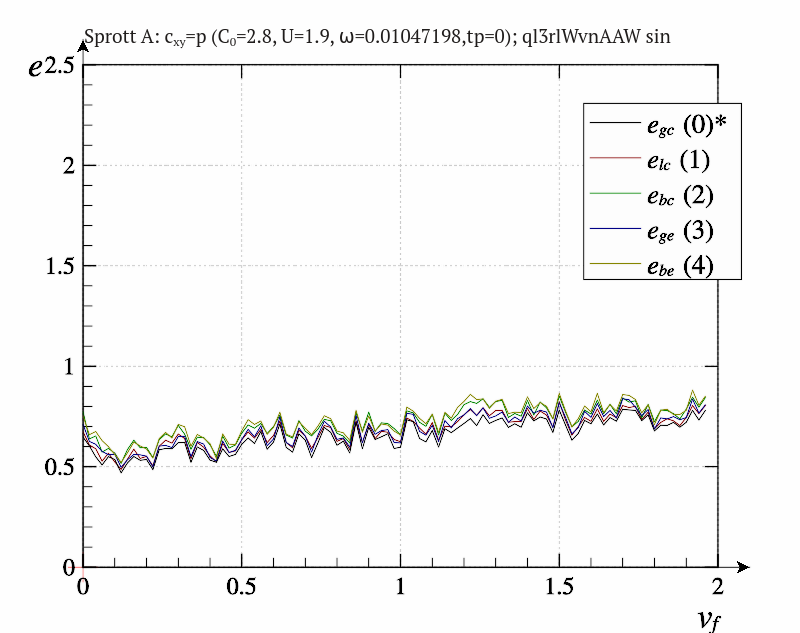
\includegraphics[width=0.49\textwidth]{p/cha/spr_a/ql3rlWvnAAW_x2/sprott_a_id-p_v_f_sin.png}
  \hfill ~
\end{center}
  \vspace{-1.0ex}
  \begin{center}
    ~ \hfill a \hfill\hfill b \hfill ~
  \end{center}
  \caption{Залежності $\overline{e} (v_f)$ при ідентифікації системи Sprott~A групою методів ql3rlWvnAAW.$q_{x^2}$ при~(\ref{atu:eq:spr_a_po_t_sign})~(a) і (\ref{atu:eq:spr_a_po_t_sin})~(b)}
  \label{atu:f:spr_a_v_f_ql3rlWvnAAW_q_x2}
\end{figure}

На рис.~\ref{atu:f:spr_a_v_f_Fq3rlFvnAAF_q_x2} представлені залежності
$\overline{e}(v_f)$ при застосуванні методів Fq3rlFvnAAF.$q_{x^2}$. Дані графіки проявляють нехай незначне, але все ж
помітна відмінність від попередніх. Для цього методу існує
слабо виражений мінімум, причому для нього
$v_f \ne 0$, що дозволяє виправдати застосування пошукового методу.

\begin{figure}[htb!]
\begin{center}
  ~ \hfill
    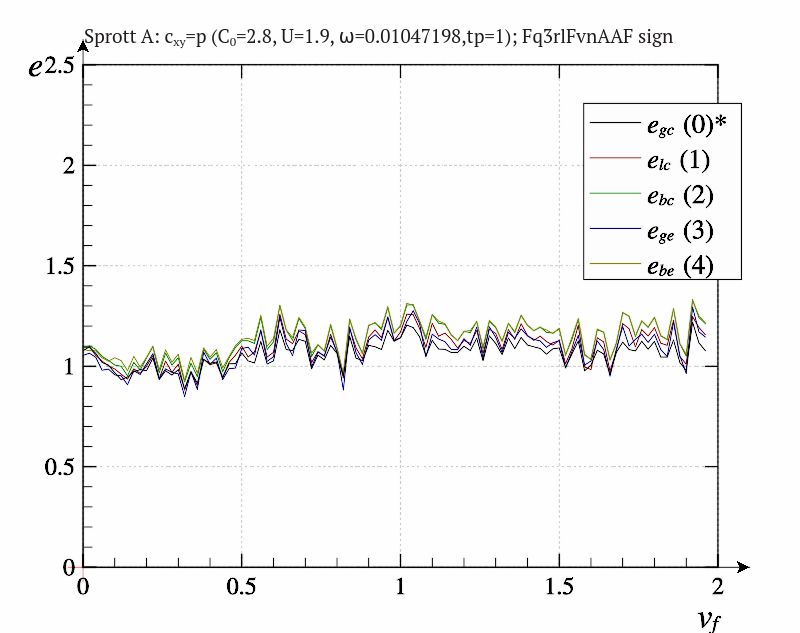
\includegraphics[width=0.49\textwidth]{p/cha/spr_a/Fq3rlFvnAAF_x2/sprott_a_id-p_v_f_sign.png}
    \hfill
    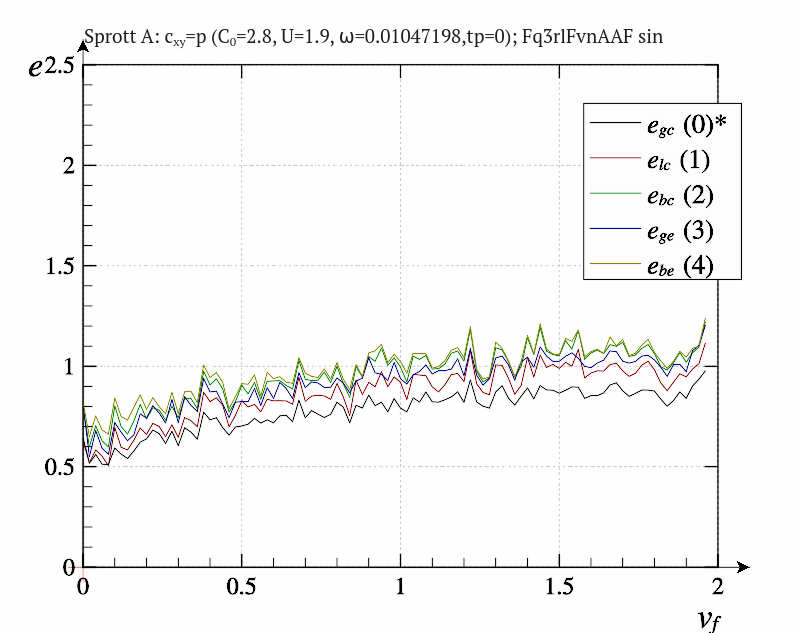
\includegraphics[width=0.49\textwidth]{p/cha/spr_a/Fq3rlFvnAAF_x2/sprott_a_id-p_v_f_sin.png}
  \hfill ~
\end{center}
\vspace{-1.5ex}
\begin{center}
  ~ \hfill a \hfill\hfill b \hfill ~
\end{center}
\vspace{-2.5ex}
  \caption{Залежності $\overline{e}(v_f)$ при ідентифікації системи Sprott~A групою методів Fq3rlFvnAAF.$q_{x^2}$ при~(\ref{atu:eq:spr_a_po_t_sign})~(a) і (\ref{atu:eq:spr_a_po_t_sin})~(b)}
  \label{atu:f:spr_a_v_f_Fq3rlFvnAAF_q_x2}
\end{figure}

Параметр
$k_e$, який визначає співвідношення сил, що діють на пошуковий
агент, для даної системи не повинен мати істотного впливу на
процес пошуку. Слабка залежність від
$v_f$ практично автоматично означає і слабку залежність від
$k_e$, так як обидва ці параметра входять у визначення однієї
і тієї ж ``сили'', що визначає зміщення пошукових агентів, а з
аналізу впливу попереднього параметра було встановлено, що в
даних конкретних умовах пошук практично не покращує результати.


На рис.~\ref{atu:f:spr_a_k_e_ql3rlWvnAAW_q_x2} представлені залежності
$\overline{e} (k_e)$ при застосуванні методу ql3rlWvnAAW.$q_{x^2}$. Переміщення агентів в процесі пошуку дозволяє зменшити
похибку ідентифікації на 10-20\%.

\begin{figure}[htb!]
\begin{center}
  ~ \hfill
    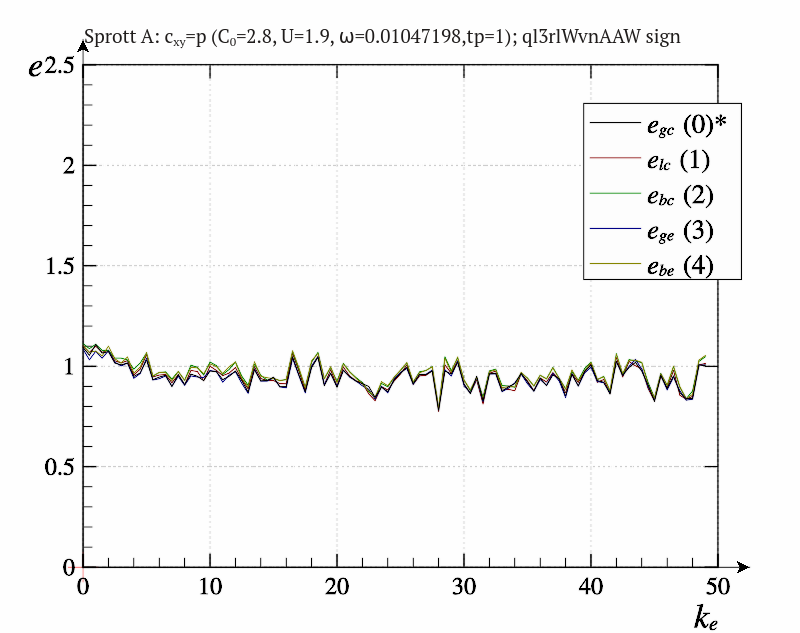
\includegraphics[width=0.49\textwidth]{p/cha/spr_a/ql3rlWvnAAW_x2/sprott_a_id-p_k_e_sign.png}
    \hfill
    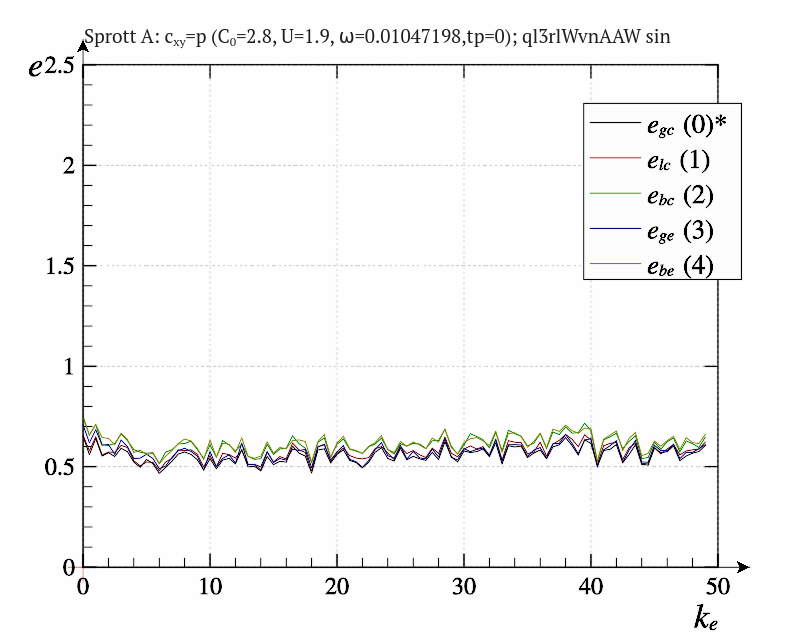
\includegraphics[width=0.49\textwidth]{p/cha/spr_a/ql3rlWvnAAW_x2/sprott_a_id-p_k_e_sin.png}
  \hfill ~
\end{center}
  \vspace{-1.0ex}
  \begin{center}
    ~ \hfill a \hfill\hfill b \hfill ~
  \end{center}
  \caption{Залежності $\overline{e} (k_e)$ при ідентифікації системи Sprott~A групою методів ql3rlWvnAAW.$q_{x^2}$ при~(\ref{atu:eq:spr_a_po_t_sign})~(a) і (\ref{atu:eq:spr_a_po_t_sin})~(b)}
  \label{atu:f:spr_a_k_e_ql3rlWvnAAW_q_x2}
\end{figure}

На рис.~\ref{atu:f:spr_a_k_e_Fq3rlFvnAAF_q_x2} представлені залежності
$\overline{e} (k_e)$ при застосуванні методів
Fq3rlFvnAAF.$q_{x^2}$.
У цьому випадку спостерігається зростання похибки
ідентифікації при зростанні
$k_e$ за умови~(\ref{atu:eq:spr_a_po_t_sin}). Динаміка агентів при цьому
стає надлишковою в порівнянні з динамікою ідентифікованого
параметра.

\begin{figure}[htb!]
\begin{center}
  ~ \hfill
    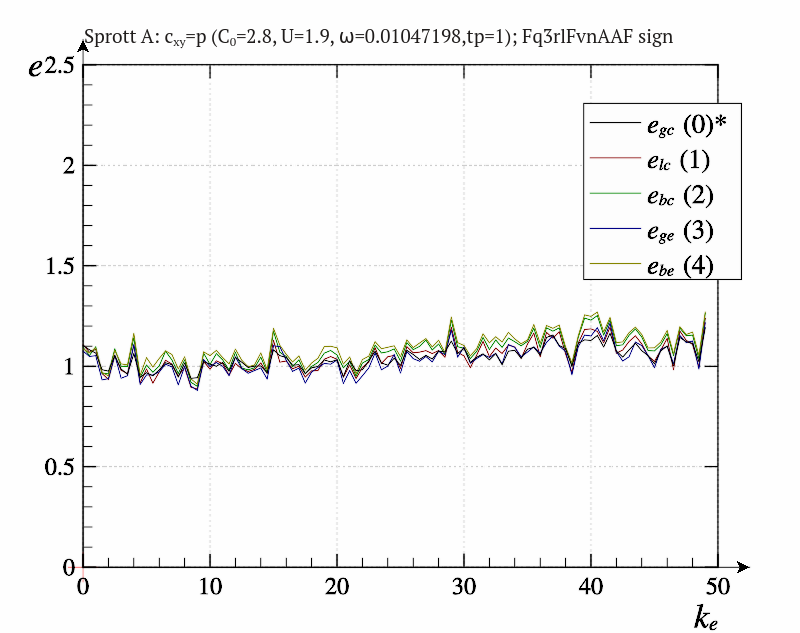
\includegraphics[width=0.49\textwidth]{p/cha/spr_a/Fq3rlFvnAAF_x2/sprott_a_id-p_k_e_sign.png}
    \hfill
    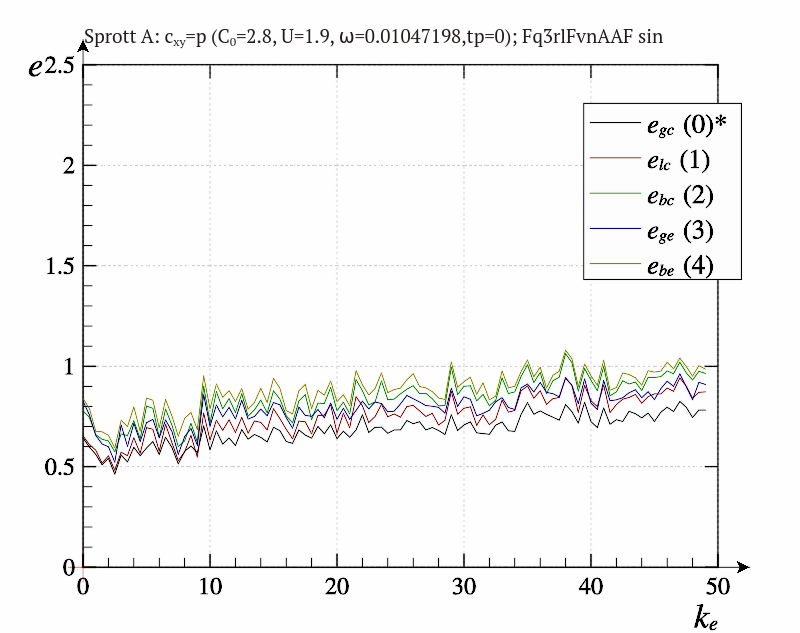
\includegraphics[width=0.49\textwidth]{p/cha/spr_a/Fq3rlFvnAAF_x2/sprott_a_id-p_k_e_sin.png}
  \hfill ~
\end{center}
  \vspace{-1.0ex}
  \begin{center}
    ~ \hfill a \hfill\hfill b \hfill ~
  \end{center}
  \caption{Залежності $\overline{e} (k_e)$ при ідентифікації системи Sprott~A групою методів Fq3rlFvnAAF.$q_{x^2}$ при~(\ref{atu:eq:spr_a_po_t_sign})~(a) і (\ref{atu:eq:spr_a_po_t_sin})~(b)}
  \label{atu:f:spr_a_k_e_Fq3rlFvnAAF_q_x2}
\end{figure}

Як і очікувалося, залежності
$\overline{e} (k_e)$ досить слабкі, і аналогічно залежностям
$\overline{e} (v_f)$, тільки для методу Fq3rlFvnAAF.
$q_{x^2}$ можна стверджувати про необхідність пошуку .

% }}}2

\subsection{Альтернативні критерії для системи Sprott~A}%{{{2

Представлені системи ідентифікації були засновані на критерії,
який були обраний шляхом перебору найбільш простих і очевидних
кандидатів. При цьому вдалося досягти працездатності систем,
однак, похибки ідентифікації були досить високі. Отже, має
сенс створити і використовувати інші критерії, використовуючи
більше інформації про систему.

В першу чергу, порівнюючи залежності
$q_{x^2}(c_{x_y})$ і
$q_{y^2}(c_{x_y})$ (рис.~\ref{atu:f:spr_a_q}), можна помітити, що піки і провали
цих залежностей близькі, а
$q_{y^2} (c_{x_y})$ в цілому практично не залежить від
$c_{x_y}$. Таким чином, можна використовувати критерій виду
%
\[
  q_{x2Oy2} = \frac{q_{x^2}}{q_{y^2}}.
\]

Далі, виходячи з виду першого з рівнянь системи~(\ref{atu:eq:spr_a})
можна зробити висновок про те, що величина
%
\begin{equation}
  q_{dxOy} =
  \frac{\overline{\dot{x}y}}{\overline{\dot{x}^2}}
  \label{atu:eq:spr_a_q_dxyOdx2}
\end{equation}
%
може бути використана в якості критерію з широким робочим
діапазоном. Під знаком усереднення мається на увазі або ковзне
середнє, або ж експоненціальне згладжування. Істотним недоліком
даного критерію є використання похідних, які як через реальних
помилок вимірювання
$x(t)$, та й та похибки оцінювання похідною схильні до стрибків
великий амплітуди. Це обмежує застосовність даного критерію
значними інтервалами оцінювання, тобто малими величинами
$a_q$.

Вид залежностей для критеріїв
$q_{x2Oy2}$ і
$q_{dxOy}$, в порівнянні з критеріями
$q_{x^2}$ і
$q_{y^2}$ представлені на рис.~\ref{atu:f:spr_a_q_alt}.

\begin{figure}[htb!]
\begin{center}
  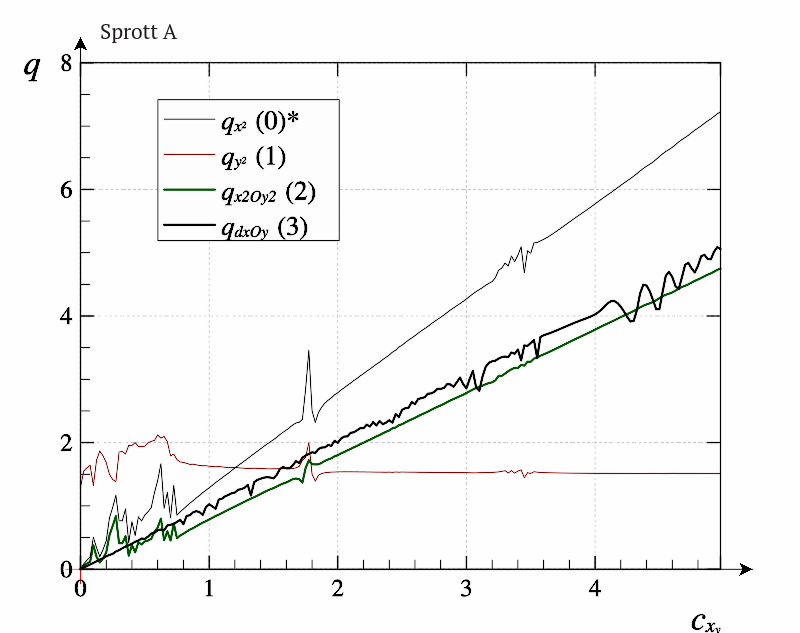
\includegraphics[width=0.60\textwidth]{p/cha/spr_a/sprott_a_q2-p_c_x_y2.png}
\end{center}
\caption{Залежності альтернативних критеріїв $q (c_{x_y})$ для системи (\ref{atu:eq:spr_a})}
\label{atu:f:spr_a_q_alt}
\end{figure}

Аналіз цих залежностей дозволяє зробити висновок про те, що
критерій
$q_{x2Oy2}$ характеризується значно меншими збуреннями, чим
початковий
$q_{x^2}$, проте ці обурення все ж присутні. При цьому зберігається
початкова ділянка з сильним порушенням монотонності. Критерій
$q_{dxOy}$ навпаки, не дивлячись на обурення, характеризується
залежністю, ближчою до лінійної, при цьому вона зберігається
як на початковій ділянці, так і в областях імпульсних збурень
інших критеріїв. Отже, цей критерій має сенс використовувати
при створенні системи ідентифікації.

Розглянемо процес ідентифікації за умов~(\ref{atu:eq:spr_a_po_t_sign}) при
використанні групи методів ql3rlWvnAAW.$q_{dxOy}$. Результати моделювання наведені на
рис.~\ref{atu:f:spr_a_id_ql3rlWvnAAW_q_dxOy_sign}.

\begin{figure}[htb!]
\begin{center}
  ~ \hfill
    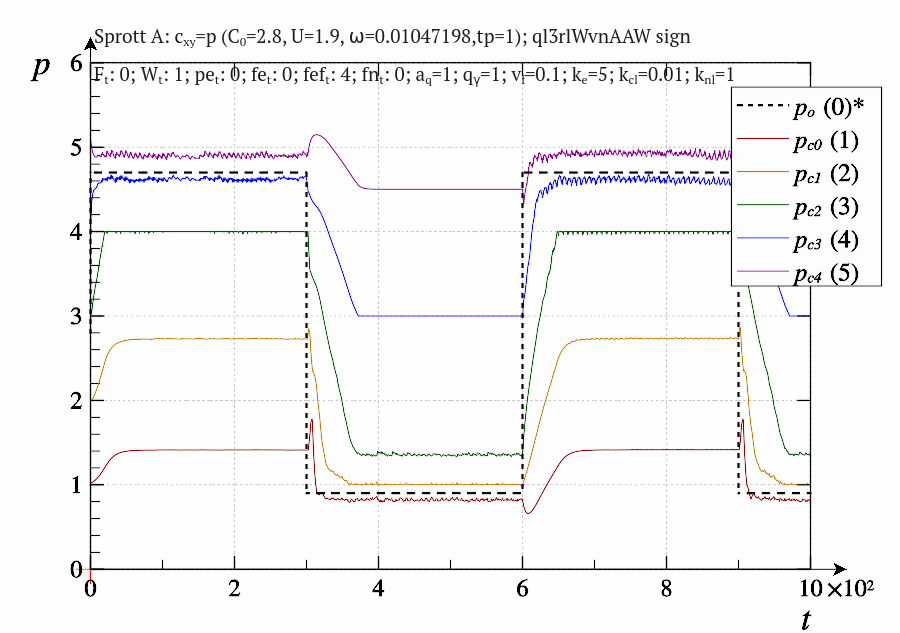
\includegraphics[width=0.49\textwidth]{p/cha/spr_a/ql3rlWvnAAW_dxOy/sprott_a_id2-p_t_pi_ql3rlWvnAAW_sign.png}
    \hfill
    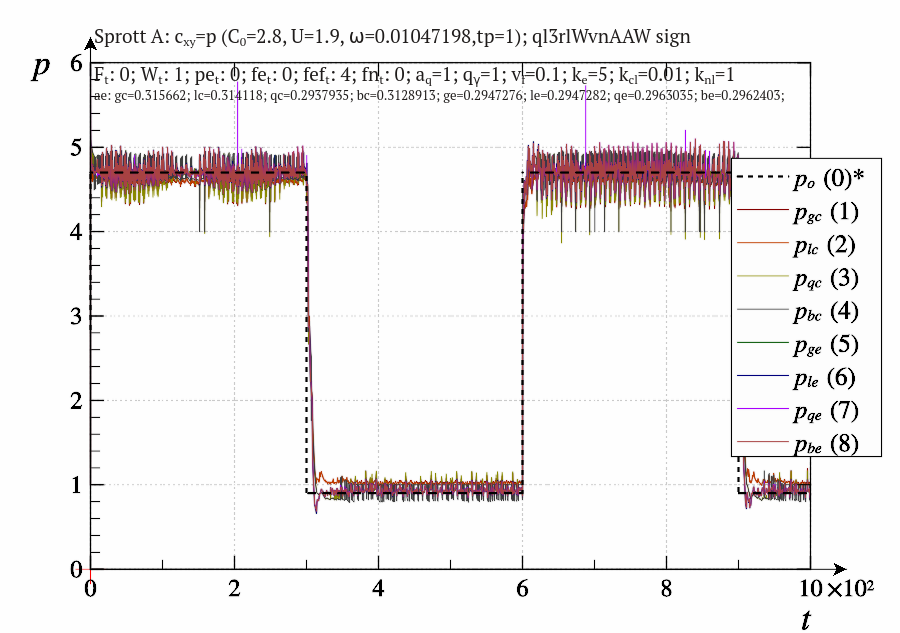
\includegraphics[width=0.49\textwidth]{p/cha/spr_a/ql3rlWvnAAW_dxOy/sprott_a_id2-p_t_p_ql3rlWvnAAW_sign.png}
  \hfill ~
\end{center}
  \vspace{-1.0ex}
  \begin{center}
    ~ \hfill a \hfill\hfill b \hfill ~
  \end{center}
  \caption{Процес ідентифікації параметра ``$c_{x_y}$'' системи Sprott~A групою методів ql3rlWvnAAW.$q_{dxOy}$ за умови~(\ref{atu:eq:spr_a_po_t_sign}): динаміка агентів~(a) та $p_\mathrm{id}$~(b)}
  \label{atu:f:spr_a_id_ql3rlWvnAAW_q_dxOy_sign}
\end{figure}

Порівнюючи ці результатів з тими, що були наведені на
рис.~\ref{atu:f:spr_a_id_ql3rlWvnAAW_q_x2_sign}, можна відзначити, що незважаючи
на збережені високочастотні коливання, рівень похибки
ідентифікації істотно зменшився.

Результати моделювання для цього ж методу,
але за умови~(\ref{atu:eq:spr_a_po_t_sin}) наведені на
рис.~\ref{atu:f:spr_a_id_ql3rlWvnAAW_q_dxOy_sin}. На відміну від методів із
застосуванням критерію
$q_{x^2}$, тут перехід до плавної зміни ідентифікованого
параметра призводить до значного зниження рівня похибки. Не
тільки зменшився розмах коливань, але і систематичні похибки
стали значно менше. Також істотно знизився час реакції на
зміну параметра.

\begin{figure}[htb!]
\begin{center}
  ~ \hfill
    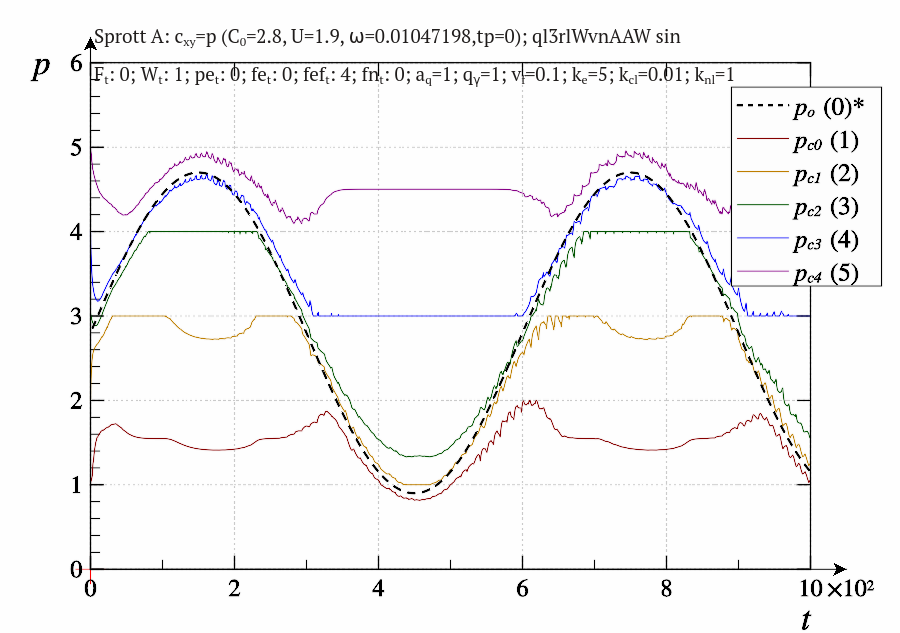
\includegraphics[width=0.49\textwidth]{p/cha/spr_a/ql3rlWvnAAW_dxOy/sprott_a_id2-p_t_pi_ql3rlWvnAAW_sin.png}
    \hfill
    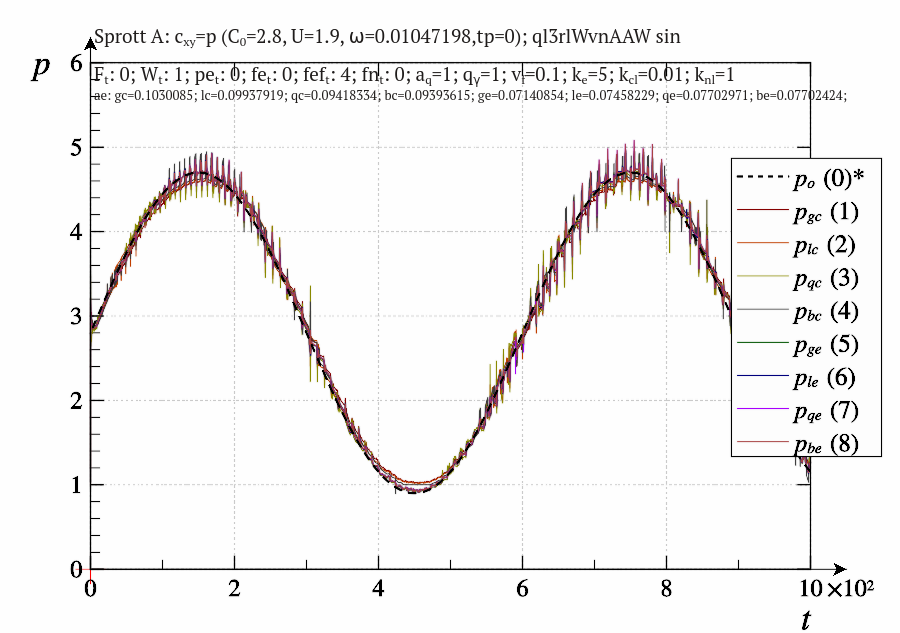
\includegraphics[width=0.49\textwidth]{p/cha/spr_a/ql3rlWvnAAW_dxOy/sprott_a_id2-p_t_p_ql3rlWvnAAW_sin.png}
  \hfill ~
\end{center}
  \vspace{-1.0ex}
  \begin{center}
    ~ \hfill a \hfill\hfill b \hfill ~
  \end{center}
  \caption{Процес ідентифікації параметра ``$c_{x_y}$'' системи Sprott~A групою методів ql3rlWvnAAW.$q_{dxOy}$ за умови~(\ref{atu:eq:spr_a_po_t_sin}): динаміка агентів~(a) та $p_\mathrm{id}$~(b)}
  \label{atu:f:spr_a_id_ql3rlWvnAAW_q_dxOy_sin}
\end{figure}

Для перевірки рівномірності ідентифікації від
значення параметра розглянемо процес ідентифікації за
умови~(\ref{atu:eq:po_t_ramp}) (рис.~\ref{atu:f:spr_a_id_ql3rlWvnAAW_q_dxOy_ramp}).

\begin{figure}[htb!]
\begin{center}
  ~ \hfill
    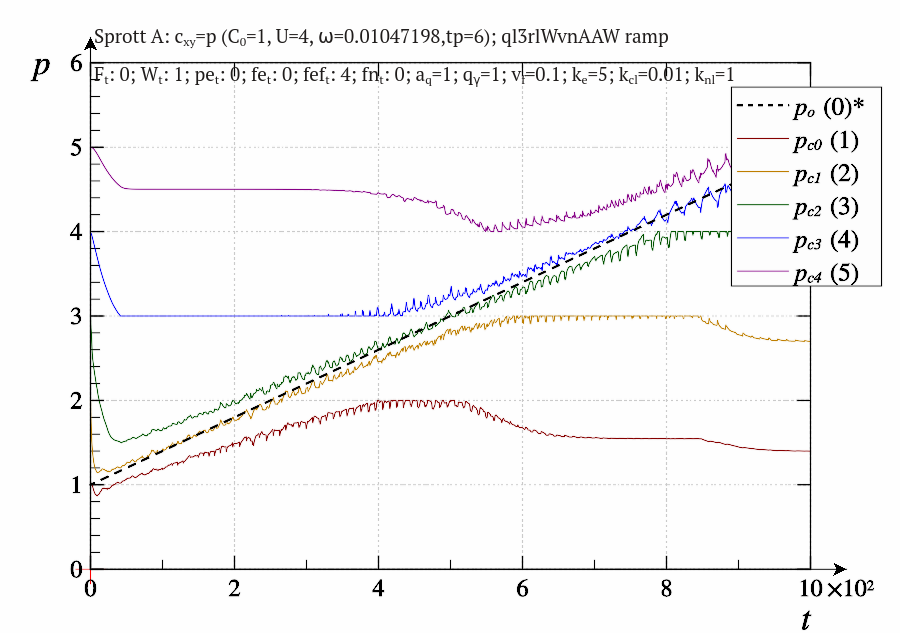
\includegraphics[width=0.49\textwidth]{p/cha/spr_a/ql3rlWvnAAW_dxOy/sprott_a_id2-p_t_pi_ql3rlWvnAAW_ramp.png}
    \hfill
    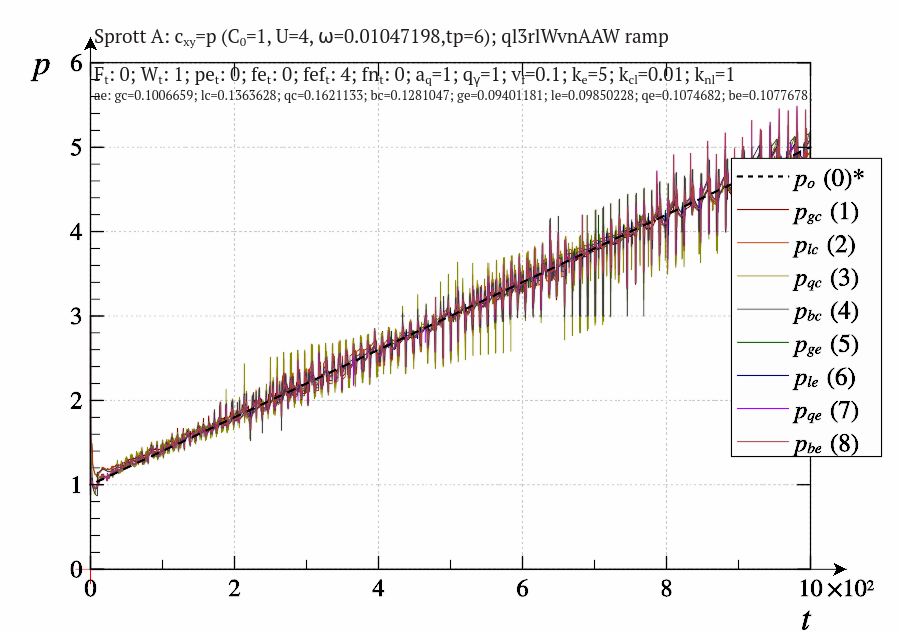
\includegraphics[width=0.49\textwidth]{p/cha/spr_a/ql3rlWvnAAW_dxOy/sprott_a_id2-p_t_p_ql3rlWvnAAW_ramp.png}
  \hfill ~
\end{center}
  \vspace{-1.0ex}
  \begin{center}
    ~ \hfill a \hfill\hfill b \hfill ~
  \end{center}
  \caption{Процес ідентифікації параметра ``$c_{x_y}$'' системи Sprott~A групою методів ql3rlWvnAAW.$q_{dxOy}$ за умови~(\ref{atu:eq:po_t_ramp}): динаміка агентів~(a) та $p_\mathrm{id}$~(b)}
  \label{atu:f:spr_a_id_ql3rlWvnAAW_q_dxOy_ramp}
\end{figure}

При порівнянні з результатами, наведеними на
рис.~\ref{atu:f:spr_a_id_ql3rlWvnAAW_q_x2_ramp}, можна зробити висновок про те, що у
всьому діапазоні зміни параметра не спостерігається помітних
відхилень
$p_\mathrm{id}$ від
$p_o$, якщо не враховувати високочастотні збурення. Вихід на
робочий режим також потребує меншого часу. Однак, імпульсні збурення
все одно присутні, хоча і в меншій мірі.

На рис.~\ref{atu:f:spr_a_a_q_ql3rlWvnAAW_q_dxOy} представлені залежності
$\overline{e}(a_q)$ при застосуванні методу
ql3rlWvnAAW.$q_{dxOy}$.
Спостерігається як загальне істотне зниження рівня похибки
ідентифікації, так обґрунтований поділ цього рівня від методу
координатора пошуку за умови~(\ref{atu:eq:spr_a_po_t_sin}). Помилка при
використанні методу
$p_{gc}$ обмежена знизу через вплив агентів, розташованих у
видаленні від
$p_o$.

\begin{figure}[htb!]
\begin{center}
  ~ \hfill
    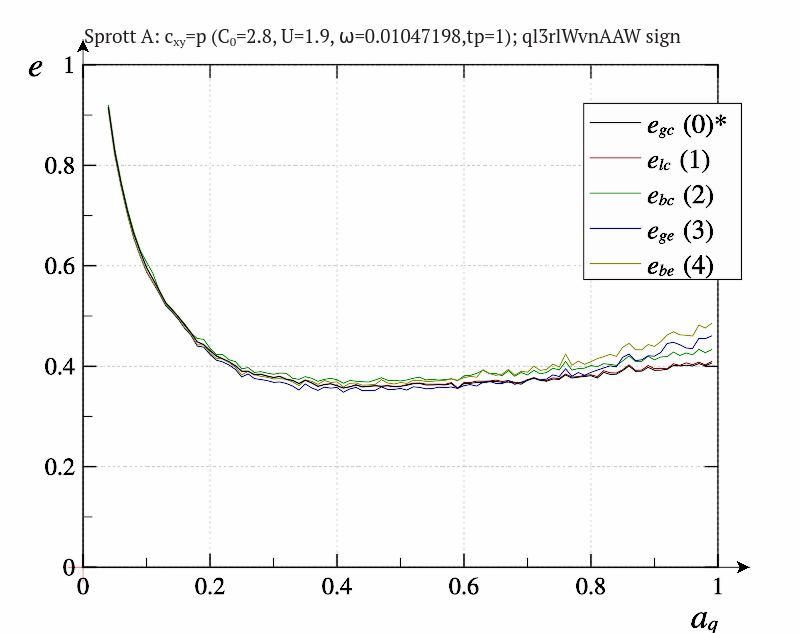
\includegraphics[width=0.49\textwidth]{p/cha/spr_a/ql3rlWvnAAW_dxOy/sprott_a_id2-p_a_q_sign.png}
    \hfill
    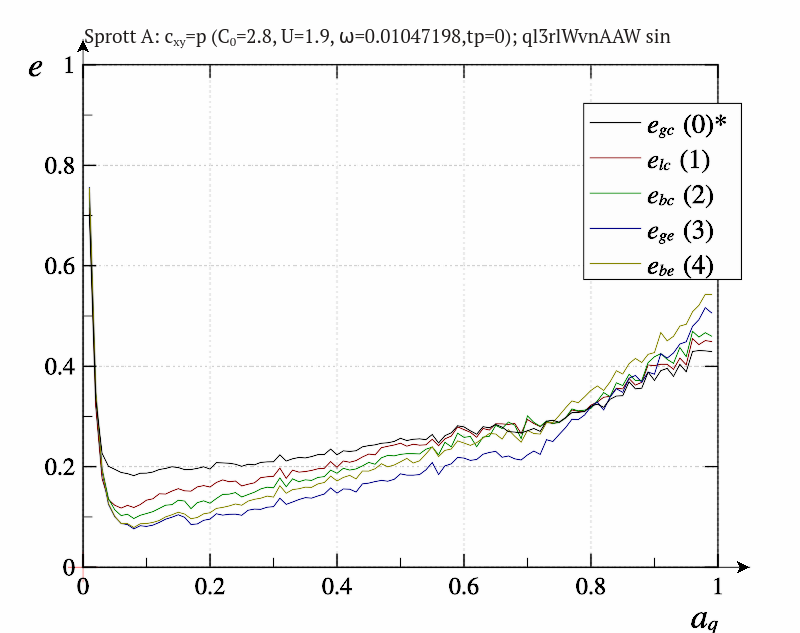
\includegraphics[width=0.49\textwidth]{p/cha/spr_a/ql3rlWvnAAW_dxOy/sprott_a_id2-p_a_q_sin.png}
  \hfill ~
\end{center}
  \vspace{-1.0ex}
  \begin{center}
    ~ \hfill a \hfill\hfill b \hfill ~
  \end{center}
  \caption{Залежності $\overline{e} (a_q)$ при ідентифікації системи Sprott~A групою методів ql3rlWvnAAW.$q_{dxOy}$ при~(\ref{atu:eq:spr_a_po_t_sign})~(a) і (\ref{atu:eq:spr_a_po_t_sin})~(b)}
\label{atu:f:spr_a_a_q_ql3rlWvnAAW_q_dxOy}
\end{figure}

На рис.~\ref{atu:f:spr_a_ql3rlWvnAAW_q_dxOy} представлені залежності
$\overline{e} (q_\gamma)$ при застосуванні групи методів
ql3rlWvnAAW.$q_{dxOy}$.

\begin{figure}[htb!]
\begin{center}
  ~ \hfill
    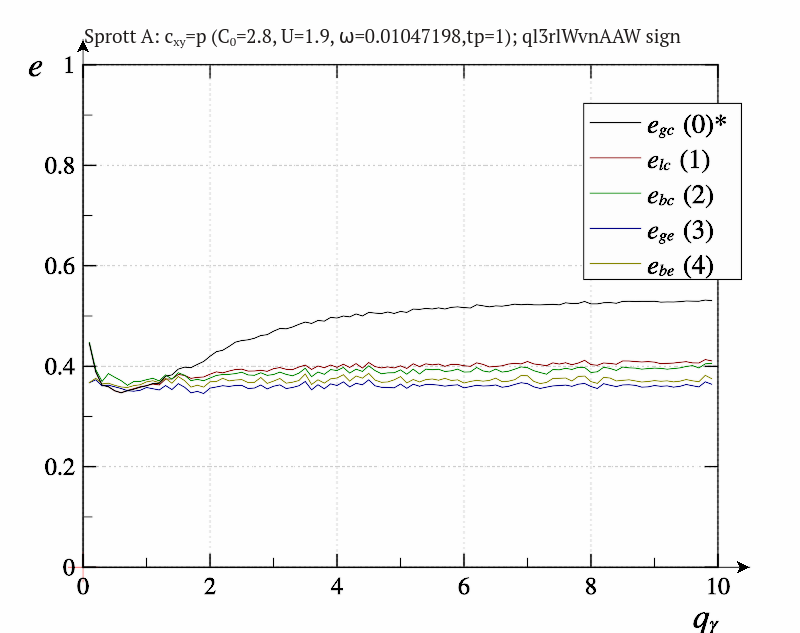
\includegraphics[width=0.49\textwidth]{p/cha/spr_a/ql3rlWvnAAW_dxOy/sprott_a_id2-p_q_gamma_sign.png}
    \hfill
    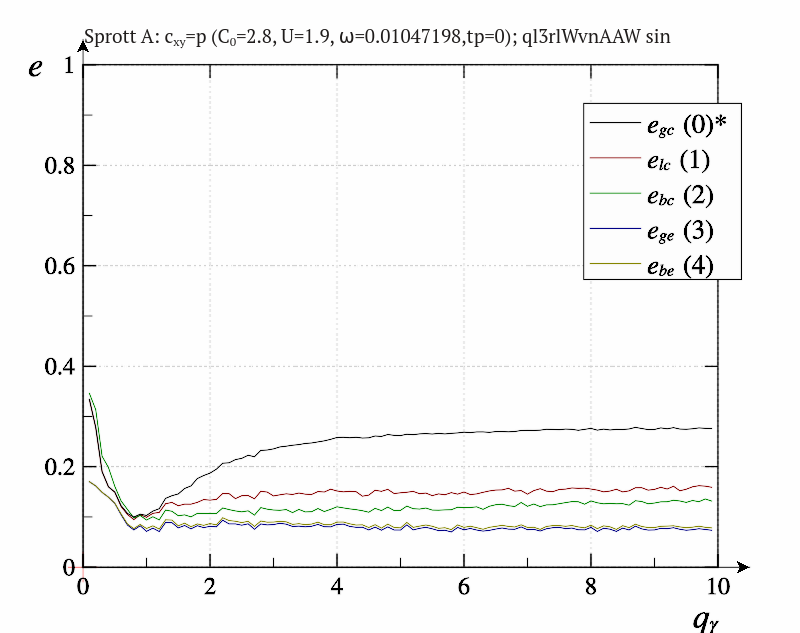
\includegraphics[width=0.49\textwidth]{p/cha/spr_a/ql3rlWvnAAW_dxOy/sprott_a_id2-p_q_gamma_sin.png}
  \hfill ~
\end{center}
  \vspace{-1.0ex}
  \begin{center}
    ~ \hfill a \hfill\hfill b \hfill ~
  \end{center}
  \caption{Залежності $\overline{e} (q_\gamma)$ при ідентифікації системи Sprott~A групою методів ql3rlWvnAAW.$q_{dxOy}$ при~(\ref{atu:eq:spr_a_po_t_sign})~(a) і (\ref{atu:eq:spr_a_po_t_sin})~(b)}
  \label{atu:f:spr_a_ql3rlWvnAAW_q_dxOy}
\end{figure}

Істотно менший рівень помилок ідентифікації, про порівнянні з
результатами, наведеними на рис.~\ref{atu:f:spr_a_qg_Fq3rlFvnAAF_q_x2} дозволяє
більш чітко виявити вплив параметра
$q_\gamma$. Явно виражений зростання похибки для всіх методів
координатора при надмірній чутливості, а також слабку
залежність для більшості методів за межами цієї зони. Виняток
становить метод
$p_{gc}$, який і повинен бути найбільш чутливими до впливу
недостатню чутливість функції якості.

На рис.~\ref{atu:f:spr_a_v_f_ql3rlWvnAAW_q_dxOy} представлені залежності
$\overline{e}(v_f)$ при застосуванні групи методів ql3rlWvnAAW.
$q_{dxOy}$. Якщо при використанні критерію
$q_{x^2}$ залежність була здебільшого умовною, то в даному випадку,
особливо за умови (\ref{atu:eq:spr_a_po_t_sin}), динаміка агентів дає істотний
внесок, зменшуючи похибку ідентифікації в 2--3 рази.

\begin{figure}[htb!]
\begin{center}
  ~ \hfill
    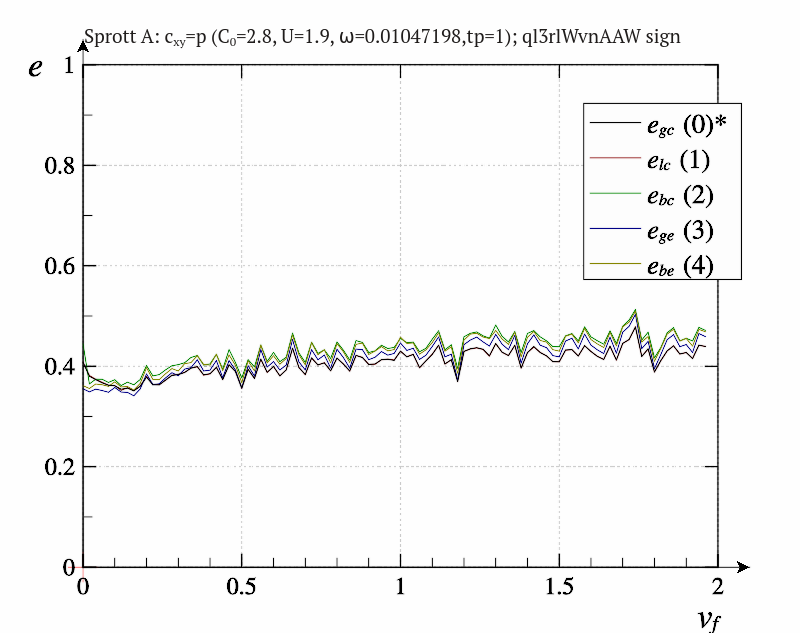
\includegraphics[width=0.49\textwidth]{p/cha/spr_a/ql3rlWvnAAW_dxOy/sprott_a_id2-p_v_f_sign.png}
    \hfill
    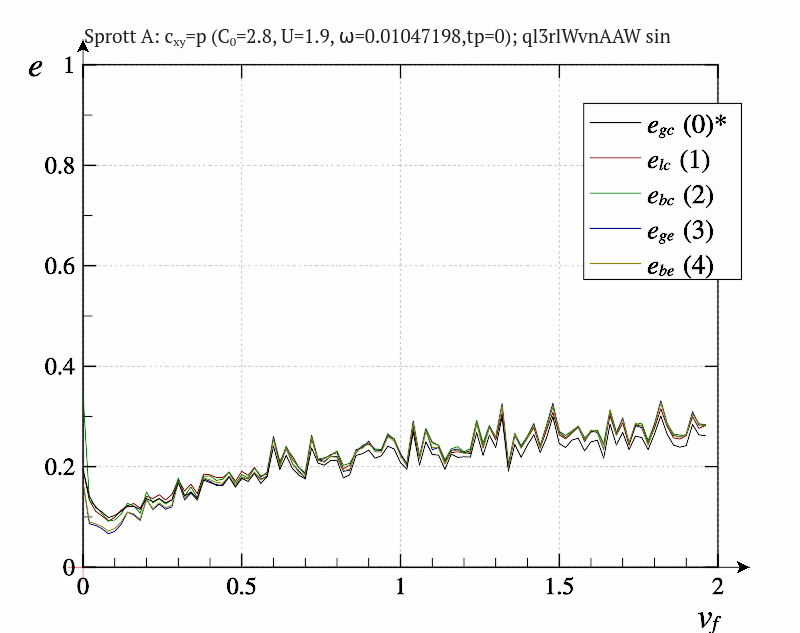
\includegraphics[width=0.49\textwidth]{p/cha/spr_a/ql3rlWvnAAW_dxOy/sprott_a_id2-p_v_f_sin.png}
  \hfill ~
\end{center}
  \vspace{-1.0ex}
  \begin{center}
    ~ \hfill a \hfill\hfill b \hfill ~
  \end{center}
  \caption{Залежності $\overline{e} (v_f)$ при ідентифікації системи Sprott~A групою методів ql3rlWvnAAW.$q_{dxOy}$ при~(\ref{atu:eq:spr_a_po_t_sign})~(a) і (\ref{atu:eq:spr_a_po_t_sin})~(b)}
  \label{atu:f:spr_a_v_f_ql3rlWvnAAW_q_dxOy}
\end{figure}

Таким чином, використання критерію
$q_{dxOy}$ дозволяє підвищити точність ідентифікації при всіх
розглянутих умовах. Недоліком є великі обчислювальні витрати
на обчислення даного критерію, але в більшості випадків це не
є проблемою.


% }}}2

\subsection{Висновки}%{{{2

В цілому, результати моделювання процесів ідентифікації системи
``Sprott~A'', і порівняння цих результатів, з даними, отриманими для
системи Лоренца, дозволяють зробити наступні висновки:

\begin{itemize}

  \item
    Спроба створити і критерій ідентифікації і працездатну систему
    ідентифікації на підставі енергетичного критерію виду
    $q_{x^2}$ виявилася успішною. Однак рівень помилок ідентифікації
    при цьому не дозволяє помітно поліпшити якість ідентифікації
    за рахунок налаштування її параметрів.

  \item
    Використання критерію
    $q_{dxOy}$ дає істотно кращі результати, і з'являється можливість
    успішно налаштовувати систему ідентифікації.

  \item
    Всі розглянуті критерії схильні до імпульсних збурень, що
    приводь до високочастотним коливанням значення
    $p_{\mathrm{id}}$.

  \item
    В цілому, використання методу ql3rlWvnleW.$q_{x^2}$
    для даної системи і початкових умов найбільш виправдано.

\end{itemize}

% }}}2


% }}}1

% vim: fdm=marker foldlevel=1 foldignore="%#" fdc=4 ft=tex
